\documentclass[11pt]{article}

\usepackage{comment} % enables the use of multi-line comments (\ifx \fi) 
\usepackage[a4paper,margin=1cm]{geometry}
\usepackage[utf8]{inputenc}
\usepackage[ngerman]{isodate}
\usepackage{gensymb}
\usepackage{graphicx}
\usepackage{booktabs}% http://ctan.org/pkg/booktabs
\usepackage{tabularx}
\usepackage{multirow}
\usepackage{ltablex} % Longtables with tabularx
\usepackage[x11names,table]{xcolor}
\usepackage{amsmath}
\usepackage{amssymb}
\usepackage{amsthm}
\usepackage{array}
\usepackage{wrapfig}
\usepackage{subcaption}
\usepackage{csquotes}
\usepackage{lscape}
\usepackage{geometry}
\usepackage{multicol}
\usepackage{bm}
\usepackage{enumitem}
\usepackage{hyperref}
\usepackage{mdframed}
\usepackage{scalerel}
\usepackage{stackengine}
\usepackage{mathtools}
\usepackage{pdfpages}

% Code highlighting
\usepackage{minted}
\surroundwithmdframed{minted}

% Be able to caption equations and float them in place
\usepackage{float}

\newmdtheoremenv{theorem}{Theorem}

\theoremstyle{definition}
\newmdtheoremenv{definition}{Definition}[section]


\geometry{a4paper, margin=2.4cm}

\newcommand\equalhat{\mathrel{\stackon[1.5pt]{=}{\stretchto{\scalerel*[\widthof{=}]{\wedge}{\rule{1ex}{3ex}}}{0.5ex}}}}
\newcommand\defeq{\mathrel{\overset{\makebox[0pt]{\mbox{\normalfont\tiny def}}}{=}}}
\newcolumntype{C}{>{\centering\arraybackslash}X}

\newcommand*\samplemean[1]{\overline{#1}}
\newcommand*\ev[1]{\mathrel{\text{E}\left[#1\right]}}
\newcommand*\R{\mathbb{R}}
\newcommand*\Z{\mathbb{Z}}
\newcommand*\N[1]{\mathcal{N}\left(#1\right)}
\newcommand*\Likelihood{\mathcal{L}}
\newcommand*\diff{\mathop{}\!\mathrm{d}}
\newcommand*\Diff[1]{\mathop{}\!\mathrm{d^#1}}
\newcommand*\Exp[1]{\mathop{\text{Exp}}\left(#1\right)}
\newcommand*\Cov[1]{\mathop{\text{Cov}}\left(#1\right)}
\newcommand*\Cor[1]{\mathop{\text{Cor}}\left(#1\right)}
\newcommand*\Var[1]{\mathop{\text{Var}}\left(#1\right)}

\DeclarePairedDelimiter\abs{\lvert}{\rvert}
\DeclarePairedDelimiter\norm{\lVert}{\rVert}

\setcounter{tocdepth}{3}
\setcounter{secnumdepth}{3}

\graphicspath{{./img/}}

\begin{document}
	
\title{Sustainable Development FS21}
\author{Pascal Baumann\\pascal.baumann@stud.hslu.ch}
\maketitle

For errors or improvement raise an issue or make a pull request on the \href{https://github.com/KilnOfTheSecondFlame/mse_summaries}{github repository}.

\tableofcontents
\newpage

\section{Sustainable Development from a Political Perspective}
\begin{quote}
	Sustainable development enables the basic needs of all people to be met and ensures a good quality of life, everywhere in the world, both now and in the future.
\end{quote}

\paragraph{Five Principles of Sustainable Development}
\begin{itemize}
	\item People\\\textit{End poverty and hunger in all forms, and ensure dignity and equality}. Ensuring that all people can be an integral part of society, that justice prevails for all and that social tensions can be kept low
	\item Prosperity\\\textit{Ensure prosperous and fulfilling lives in harmony with nature}. Ensuring that all people are able to achieve a standard of living that meets at least their basic needs
	\item Peace\\\textit{Foster peaceful, just and inclusive societies}. Ensuring that peaceful and inclusive societies can emerge
	\item Partnership\\\textit{Implement the agenda through a solid global partnership}. Ensuring that all interests are taken into account in decision-making processes and that no one is left out or left behind
	\item Planet\\\textit{Protect our planet's natural resources and climate for future generations}. Ensuring that planetary boundaries are respected
\end{itemize}

\paragraph{Integrated, Equal and Balanced}
\begin{itemize}
	\item \textbf{Integrated}\\
	Only through intact natural resources an efficient economy can emerge. Only through an intact economy prosperity can be created. This prosperity can only be distributed fairly in a society based on solidarity. Political processes can be designed in such a way that natural resources are preserved in the long term
	\item \textbf{Equal}\\
	All three dimensions are of equal importance
	\item \textbf{Balanced}\\
	If equal consideration is not possible in specific contexts or in relation to specific problems, deficits in disadvantaged dimensions are to be compensated
\end{itemize}

\begin{figure}[H]
	\centering
	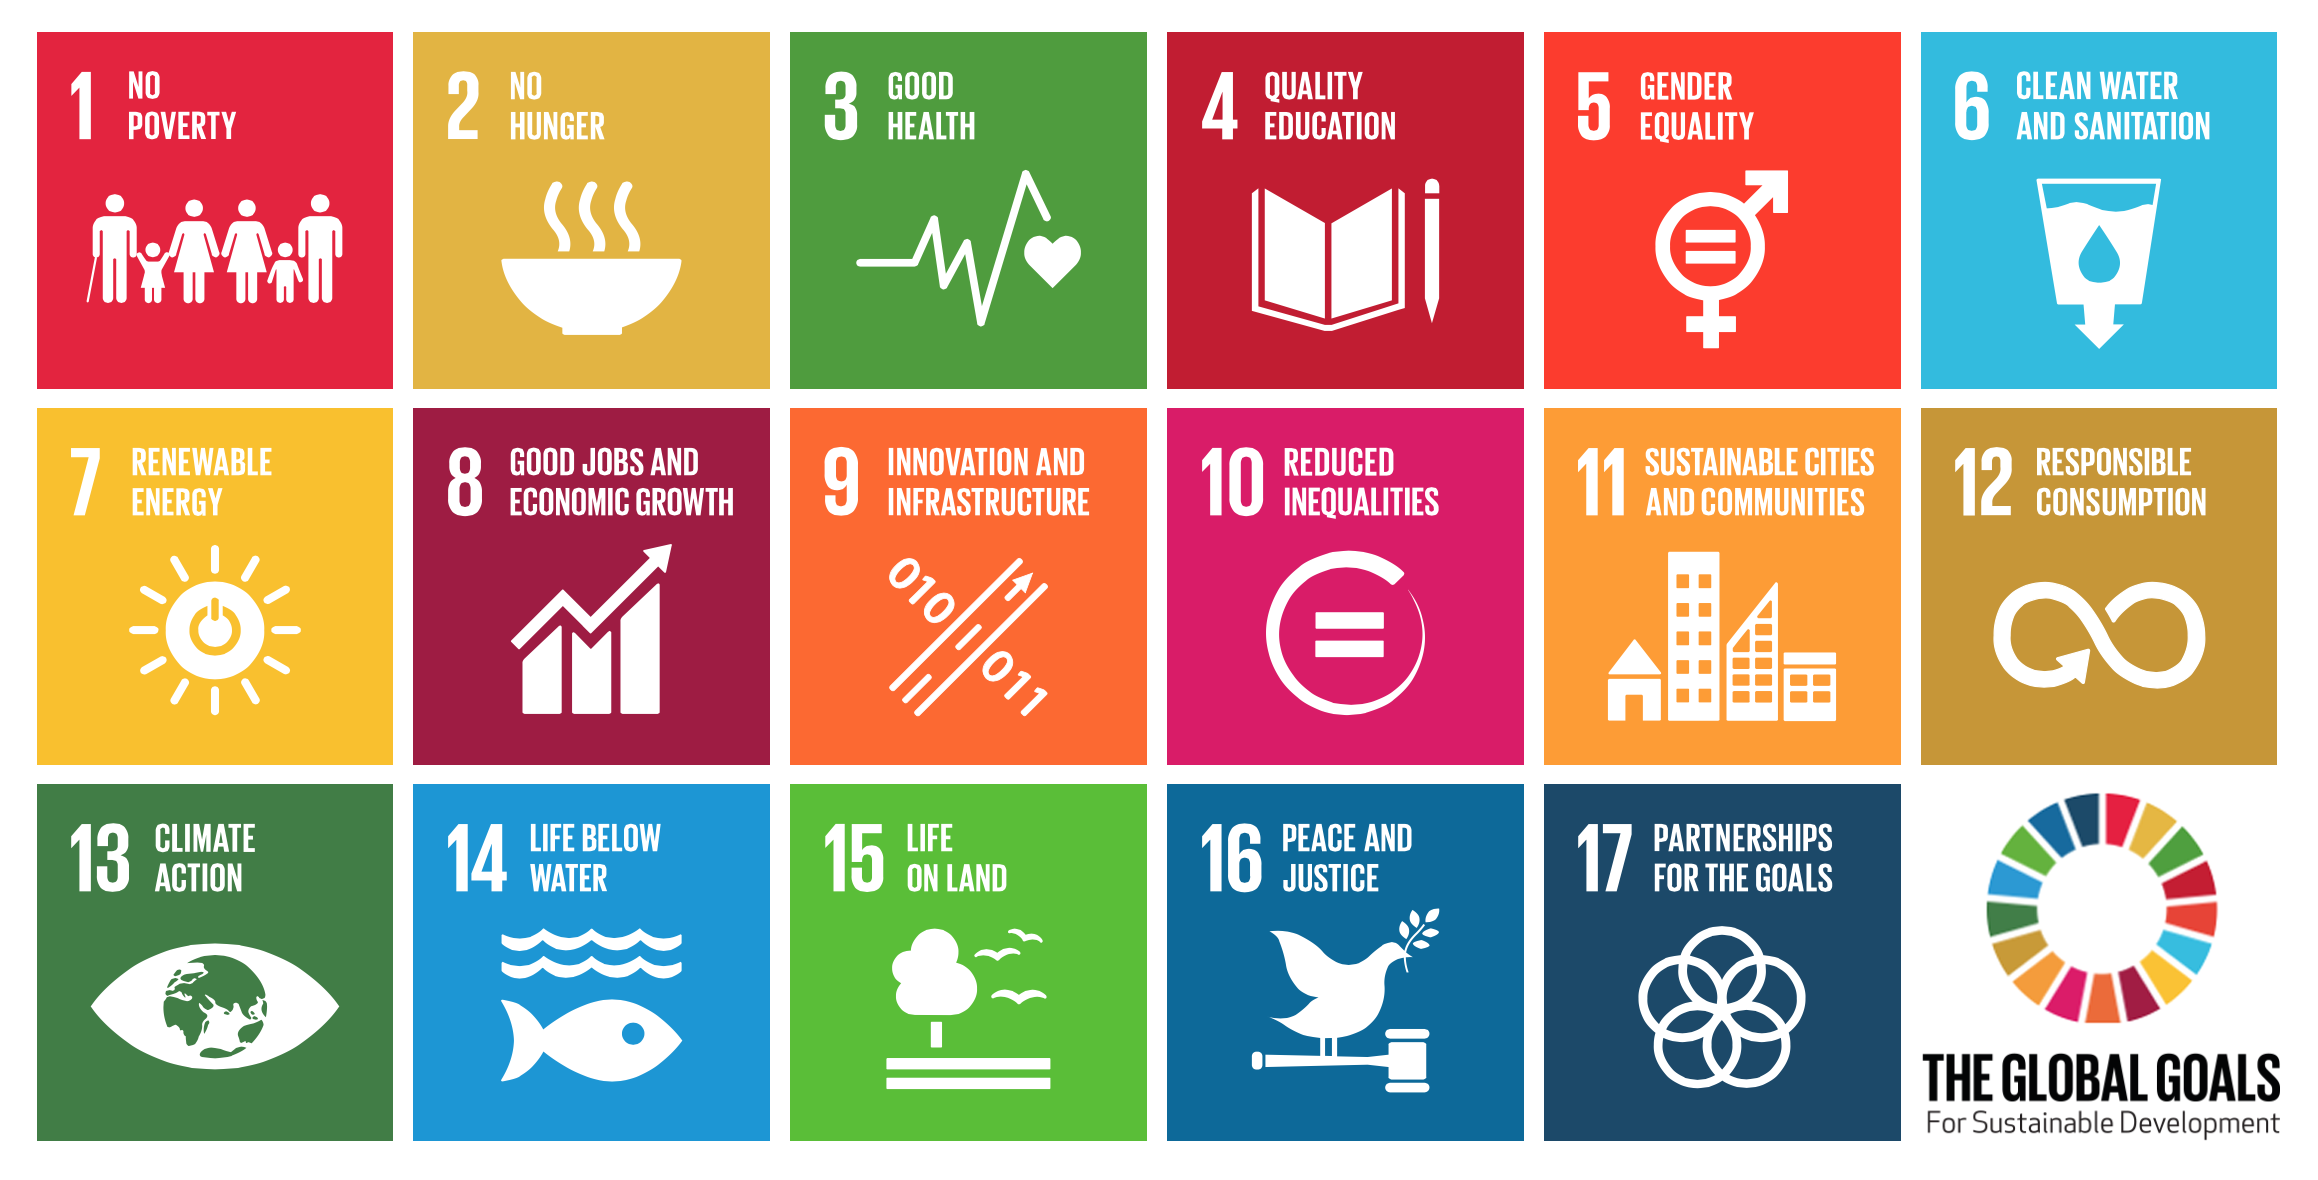
\includegraphics[width=0.9\linewidth]{img/sustainable_development_goals}
	\caption{United Nations Sustainable Development Goals}
	\label{fig:sustainabledevelopmentgoals}
\end{figure}

\begin{figure}[H]
	\centering
	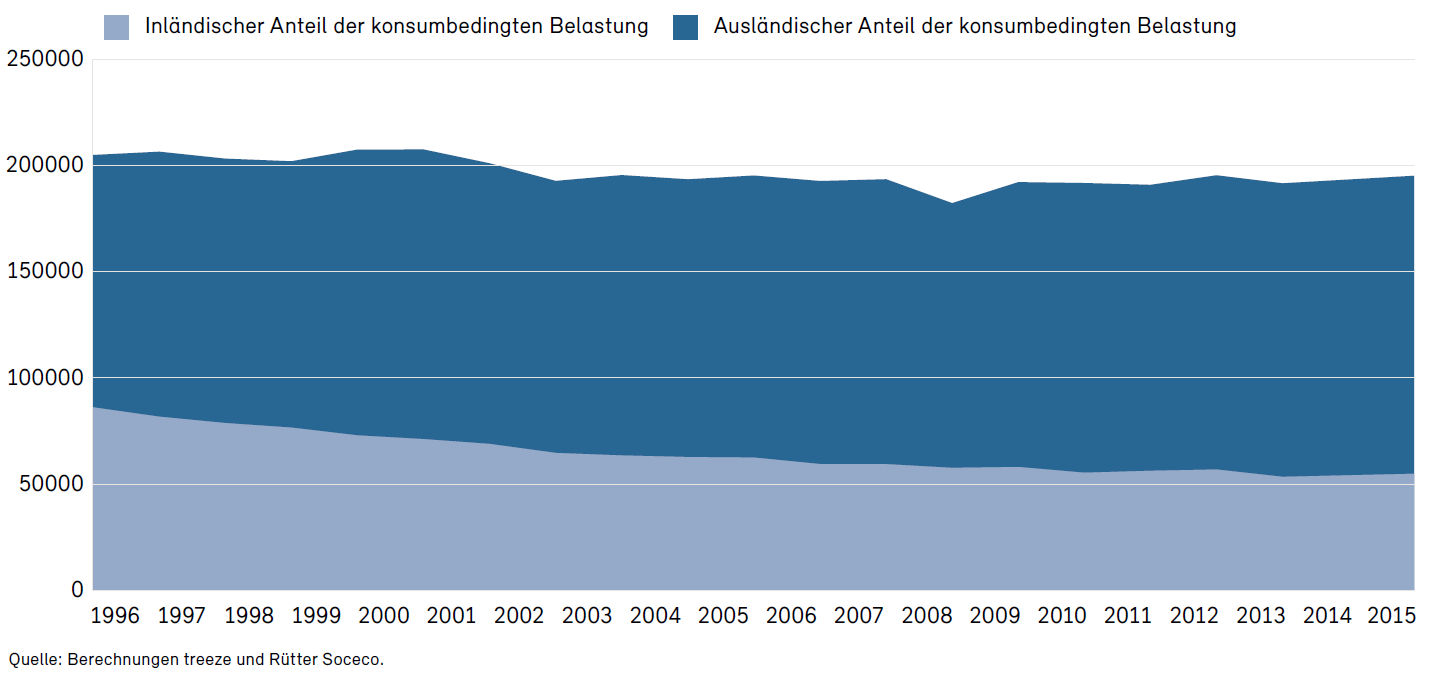
\includegraphics[width=0.8\linewidth]{img/environmental_impact_switzerland}
	\caption{Switzerland exports more than 70\% of its environmental impact (BAFU, Umweltfussabdrücke Schweiz, 2018).}
	\label{fig:environmentalimpactswitzerland}
\end{figure}

Sustainable development affects almost all areas of our society. The added value of a meta-perspective like the SDG is:
\begin{itemize}
	\item Orientation\\
	Clear objectives indicate where the path should lead and how far it still has to go. They point out the need for action and urgencies, and set priorities.
	\item Policy coherence\\
	The goals are interrelated and must be solved together. The meta-strategy helps to see the connections and address them together.
\end{itemize}

\section{Fundamentals of Sustainable Development}

\begin{quote}
	\textquotedblleft If the present growth trends in world population, industrialization, pollution, food production, and resource depletion continue unchanged, the limits to growth on this planet will be reached sometime within the next one hundred years. The most probable result will be a rather sudden and uncontrollable decline in both population and industrial capacity.\textquotedblright
\end{quote}

\begin{quote}
	\textquotedblleft Sustainable development is development that meets the needs of the present without compromising the ability of future generations to meet their own needs.\textquotedblright
\end{quote}

\begin{figure}[H]
	\centering
	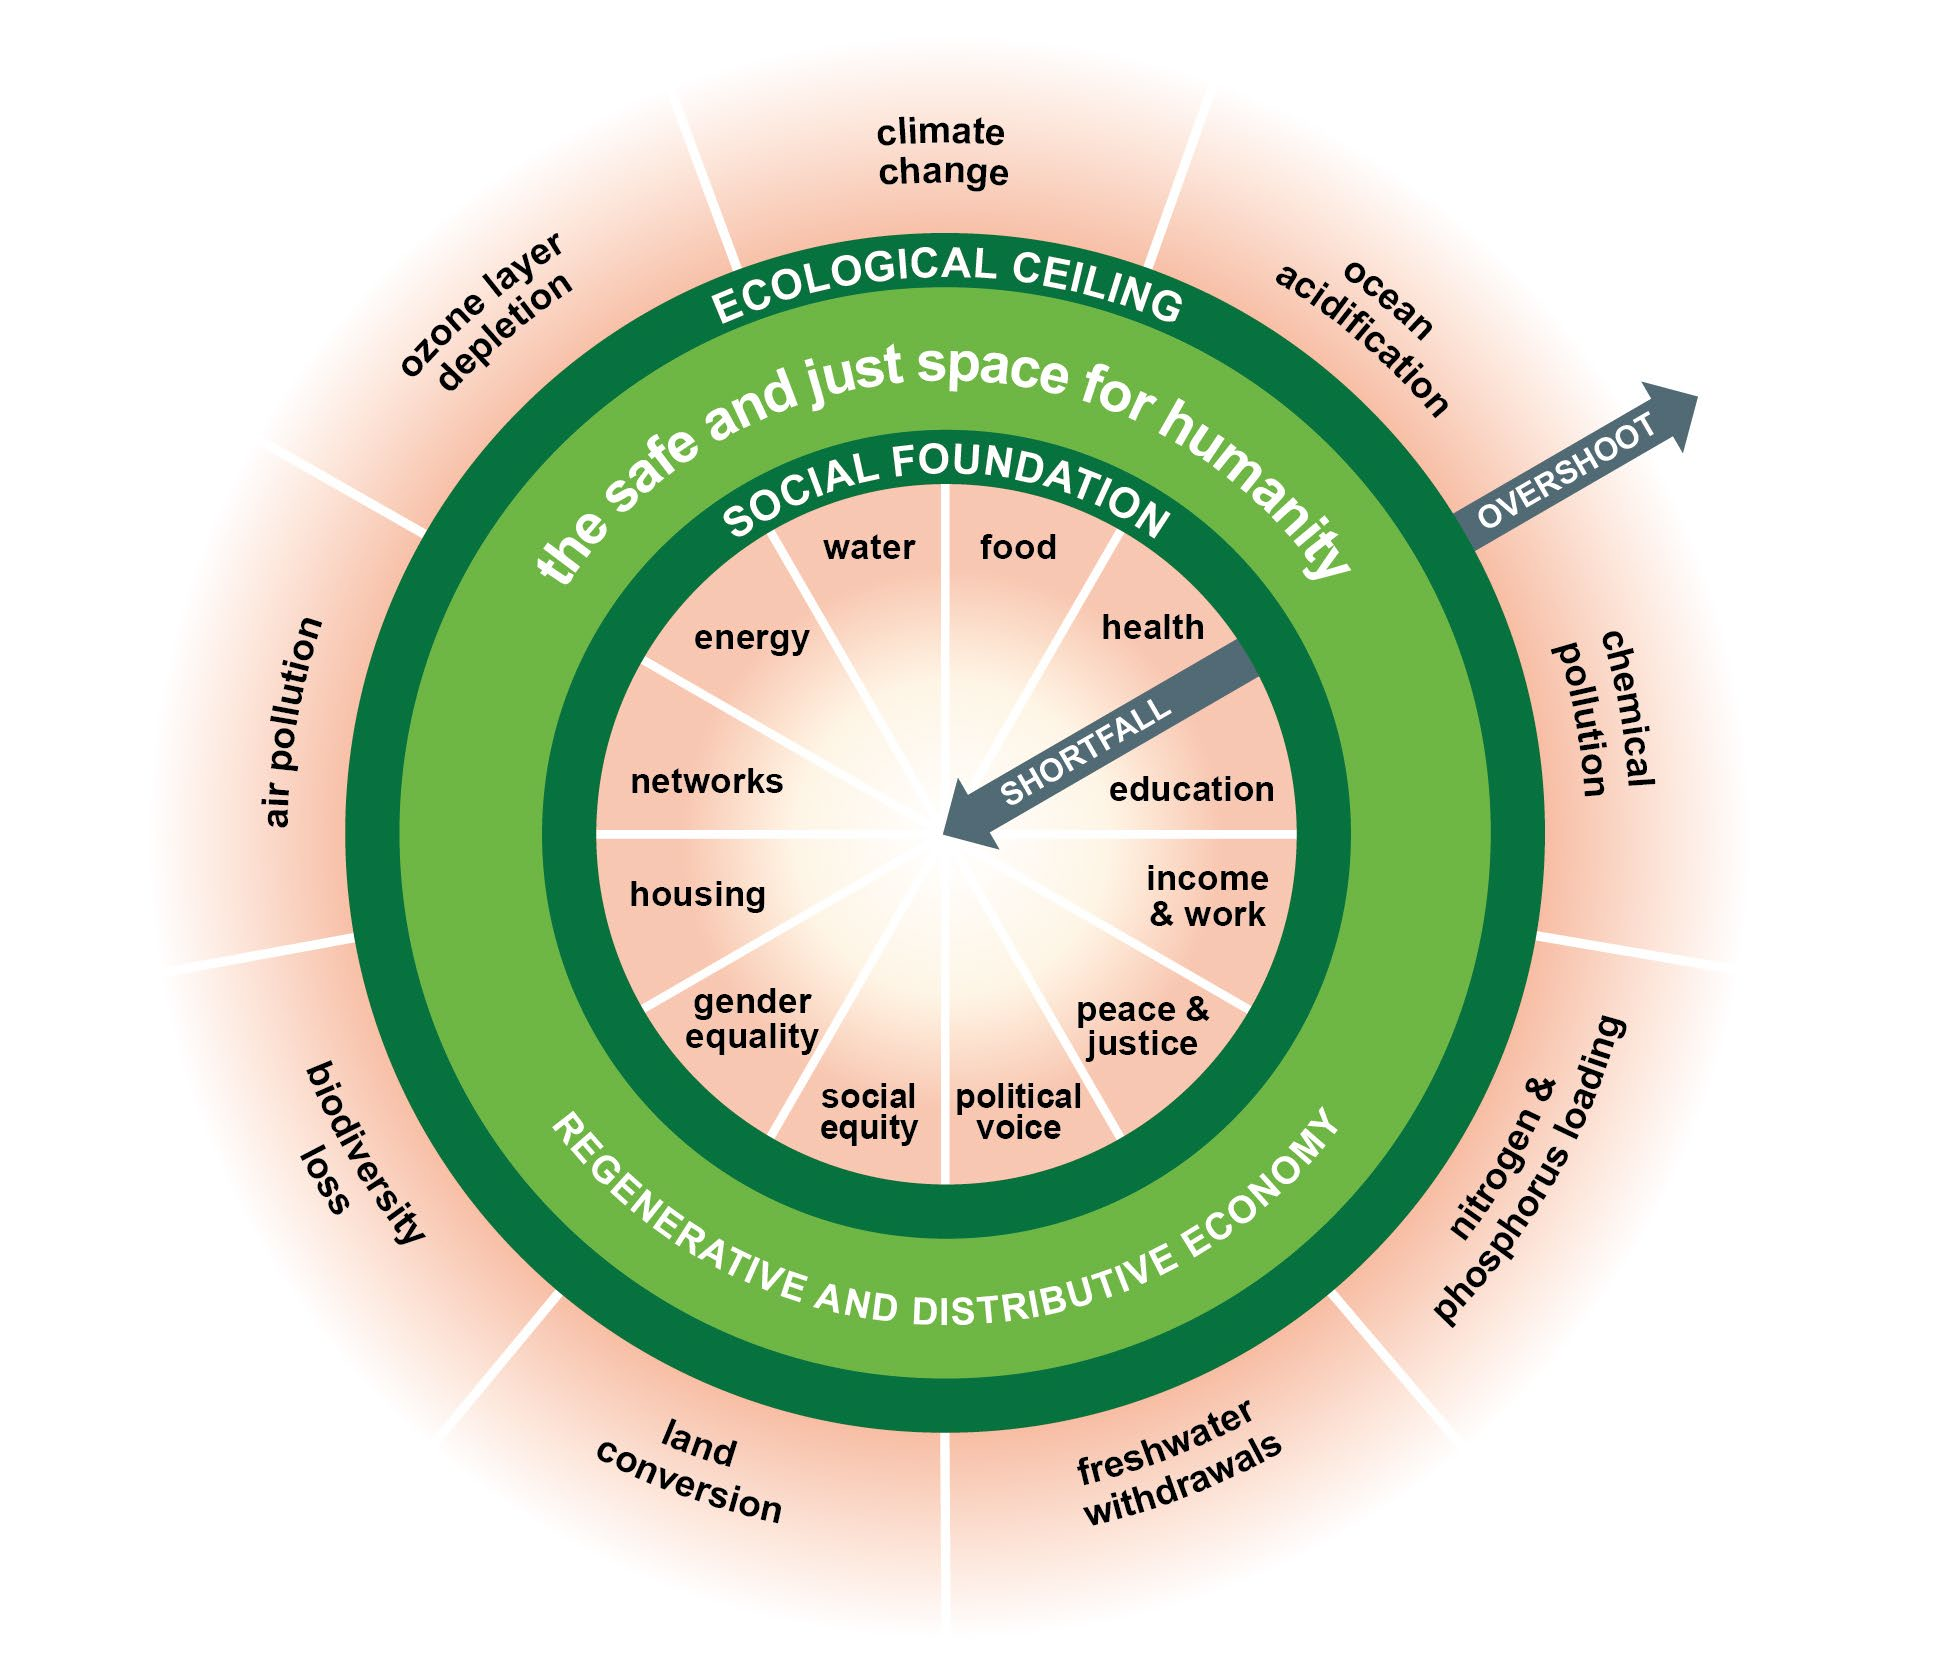
\includegraphics[width=0.6\linewidth]{img/doughnut_model.png}
	\caption{The doughnut model for sustainable development}
\end{figure}

\begin{figure}[H]
	\centering
	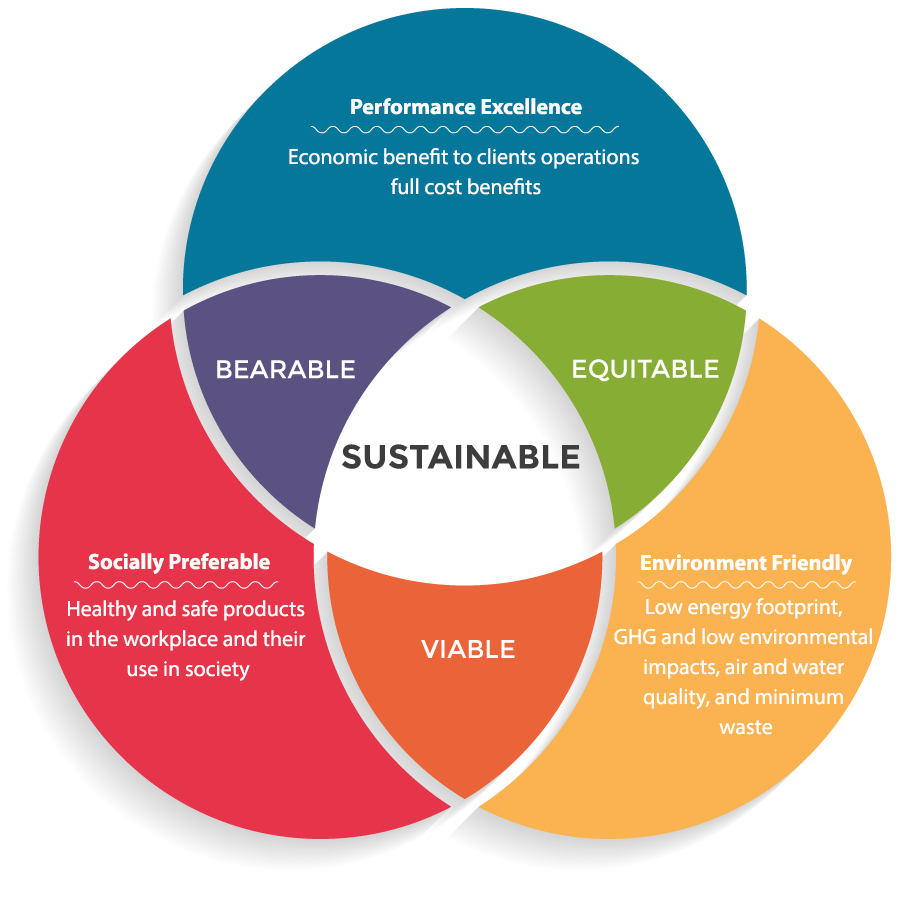
\includegraphics[width=0.5\linewidth]{img/triple_bottom_line.png}
	\caption{The triple bottom line concept for sustainable development}
\end{figure}

\subsection{International Debate}

\subsubsection{Six Core Functions of International Conferences on Sustainable Development}
\begin{itemize}[noitemsep]
	\item \textbf{Setting Global Agendas}
	\begin{itemize}
		\item Providing a relatively open space in which states, international organizations, and NGOs can meet to plan the future trajectory of sustainable development
		\item Addressing, discussing and resolving global issues of sustainable development
		\item Creating and increasing political, media and public attention
	\end{itemize}
	\item \textbf{'Joining up' Problems}
	\begin{itemize}
		\item Bringing together debates on global long-term issues that are often dealt with in a disconnected and ad hoc manner (e.g., poverty, inequality, environmental protection, development priorities)
		\item Addressing the contradictions between the different target dimensions by developing and promoting integrative concepts
	\end{itemize}
	\item \textbf{Endorsing Common Principles}
	\begin{itemize}
		\item Signing of (binding) agreements and resolutions that provide guidelines, recommendations and standards
		\item "Soft law" that in time, hopefully, will become "hard law"
	\end{itemize}
	\item \textbf{Providing Leadership}
	\begin{itemize}
		\item World leaders meeting to address issues that cannot be adequately dealt with at lower levels of governance
		\item Defining objectives for action at lower tiers of governance
	\end{itemize}
	\item \textbf{Capacity Building}
	\begin{itemize}
		\item Creation of new international organizations like the UN Environment Programme (UNEP), UN High-level Political Forum on Sustainable Development (HLPF)
		\item Stimulating the formation of environmental ministries, action plans etc. at the national level
		\item Providing key yardsticks to increase engagement at the national level
		\item Contributing to a process of societal and institutional change
	\end{itemize}
	\item \textbf{Fostering Inclusiveness and Legitimacy}
	\begin{itemize}
		\item Delegations from all UN member states
		\item High number of Heads of State and Government
		\item Participation of “major groups” and other stakeholders
	\end{itemize}
\end{itemize}

\subsection{Agenda 2030 for Sustainable Development}
Signed by all 193 UN member countries with the overarching aim for a fundamental social, economic and environmental transformation. This resolution is not legally binding and only a declaration of intent. There are contradictory goals, promote economic and social development while reducing the impact on the environment at the same time. And scientific and technological innovation is seen as a key enabler of sustainable development. Monitoring and reviewing of target achievement based on a set of indicators on global and national level.

\begin{figure}[H]
	\centering
	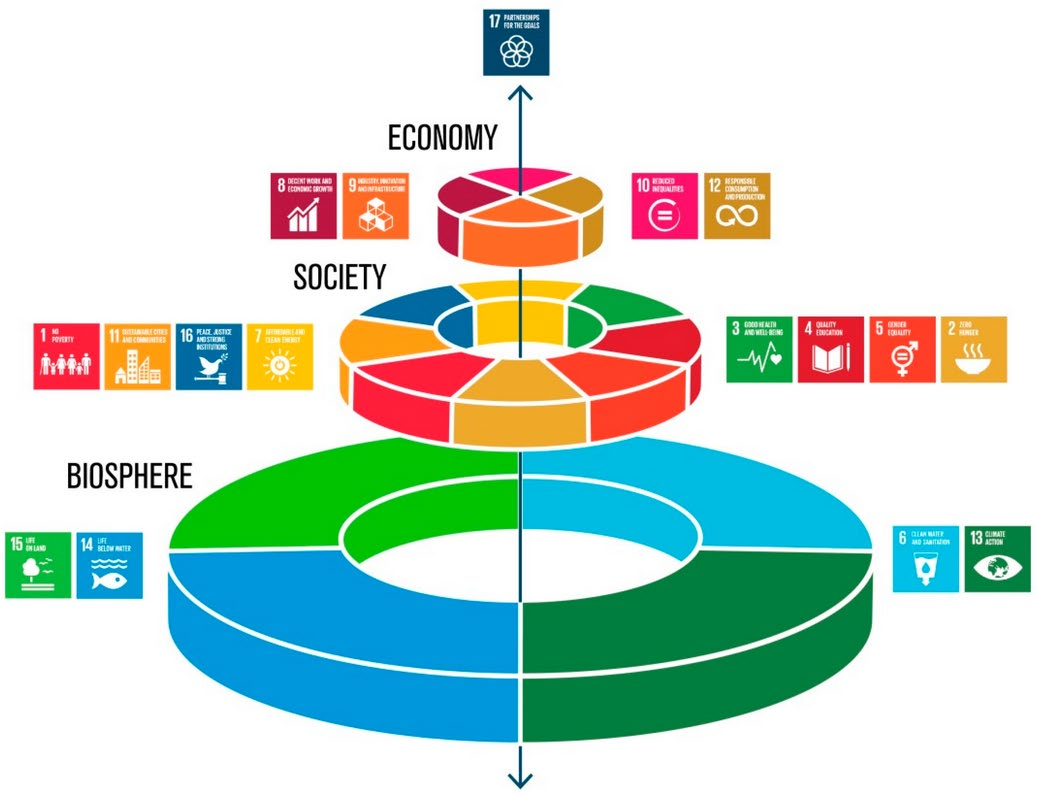
\includegraphics[width=0.6\linewidth]{img/tripartite_model_sustainability}
	\caption{Sustainable Development Goals and tripartite model of sustainability}
	\label{fig:tripartitemodelsustainability}
\end{figure}

The Paris Agreement is a document with crucial areas necessary to combat climate change, and this commitment is legally binding.

\begin{figure}[H]
	\centering
	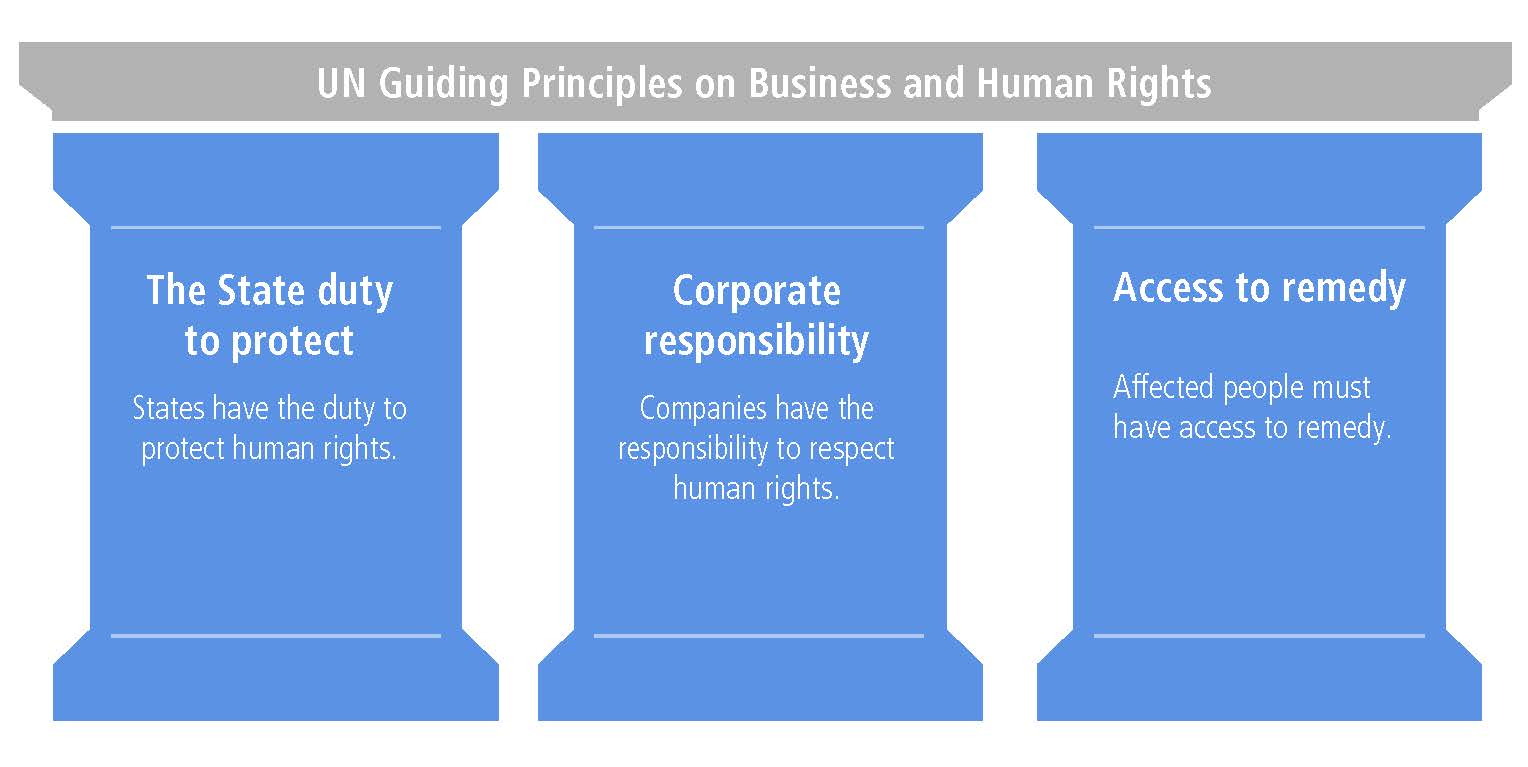
\includegraphics[width=0.8\linewidth]{img/principles_business_human_rights}
	\caption{UN guiding principles on business and human rights}
	\label{fig:principlesbusinesshumanrights}
\end{figure}

\begin{itemize}
	\item Protect human rights through effective policies, legislation, regulations and adjudication
	\item States need to set out the expectation that all business organisations respect human rights throughout their operations
	\item Companies should avoid infringing on the human rights of others
	\item Companies should avoid causing or contributing to and seek to prevent or mitigate adverse human rights impacts through their own activities and address such impacts when they occur
	\item Companies should have policies and processes appropriate to their size and circumstances
	\item States must take appropriate steps to ensure, through judicial, administrative, legislative or other appropriate means, that when such abuses occur within their territory or jurisdiction those affected have access to effective remedy
\end{itemize}

\subsection{Guidelines for Businesses}
\begin{itemize}
	\item OECD Guidelines for Multinational Enterprises
	\begin{itemize}
		\item Published by Organization for Economic Cooperation and Development (OECD)
		\item Recommendations for responsible business conduct for multinational enterprises
		\item Topics include information disclosure, human rights, labour relations, the environment, fighting corruption, consumer interests, science and technology, competition and taxation
		\item Signatory states are required to establish a National Contact Point (NCP) that promotes the implementation of the guidelines and addresses reports of alleged violations
	\end{itemize}
	\item OECD Anti-Bribery Convention
	\begin{itemize}
		\item Published by Organization for Economic Cooperation and Development (OECD)
		\item Include legally binding standards to criminalize bribery of foreign public officials
		\item Focus on the supply side of bribery, that is voluntarily or not give the bribe
		\item Legally binding and signatories must establish that the bribery of foreign officials is a crime in the national legal framework, and must provide means and measures to prevent, detect, investigate, prosecute and sanction foreign bribery
	\end{itemize}
	\item ISO 14001 - Environmental Management
	\begin{itemize}
		\item Published by the International Organization for Standardization
		\item Practical tools to manage environmental responsibilities, to set up an effective environmental management system
		\item Mentions audits, communications, labelling and life cycle analysis, environmental challenges such as climate change
		\item Not legally binding but companies can be certified by the ISO
	\end{itemize}
	\item ISO 26000 - Social Responsibility
	\begin{itemize}
		\item Published by the International Organization for Standardization
		\item Guiding principles for social responsibility at organizations
		\item Organization management, human rights, working practices, the environment, fair corporate and business practices, consumer affairs, involvement and development of local communities
		\item Not legally binding, not certifiable
	\end{itemize}
	\item Global Reporting Initiative (GRI) Standards Glossary
	\begin{itemize}
		\item Guiding principles for sustainability reporting
		\item Targeted towards enterprises and other organizations
		\item Comprehensive framework for sustainability reporting
		\item Not legally binding
	\end{itemize}
\end{itemize}

\subsection{National Debate}

\begin{figure}[H]
	\centering
	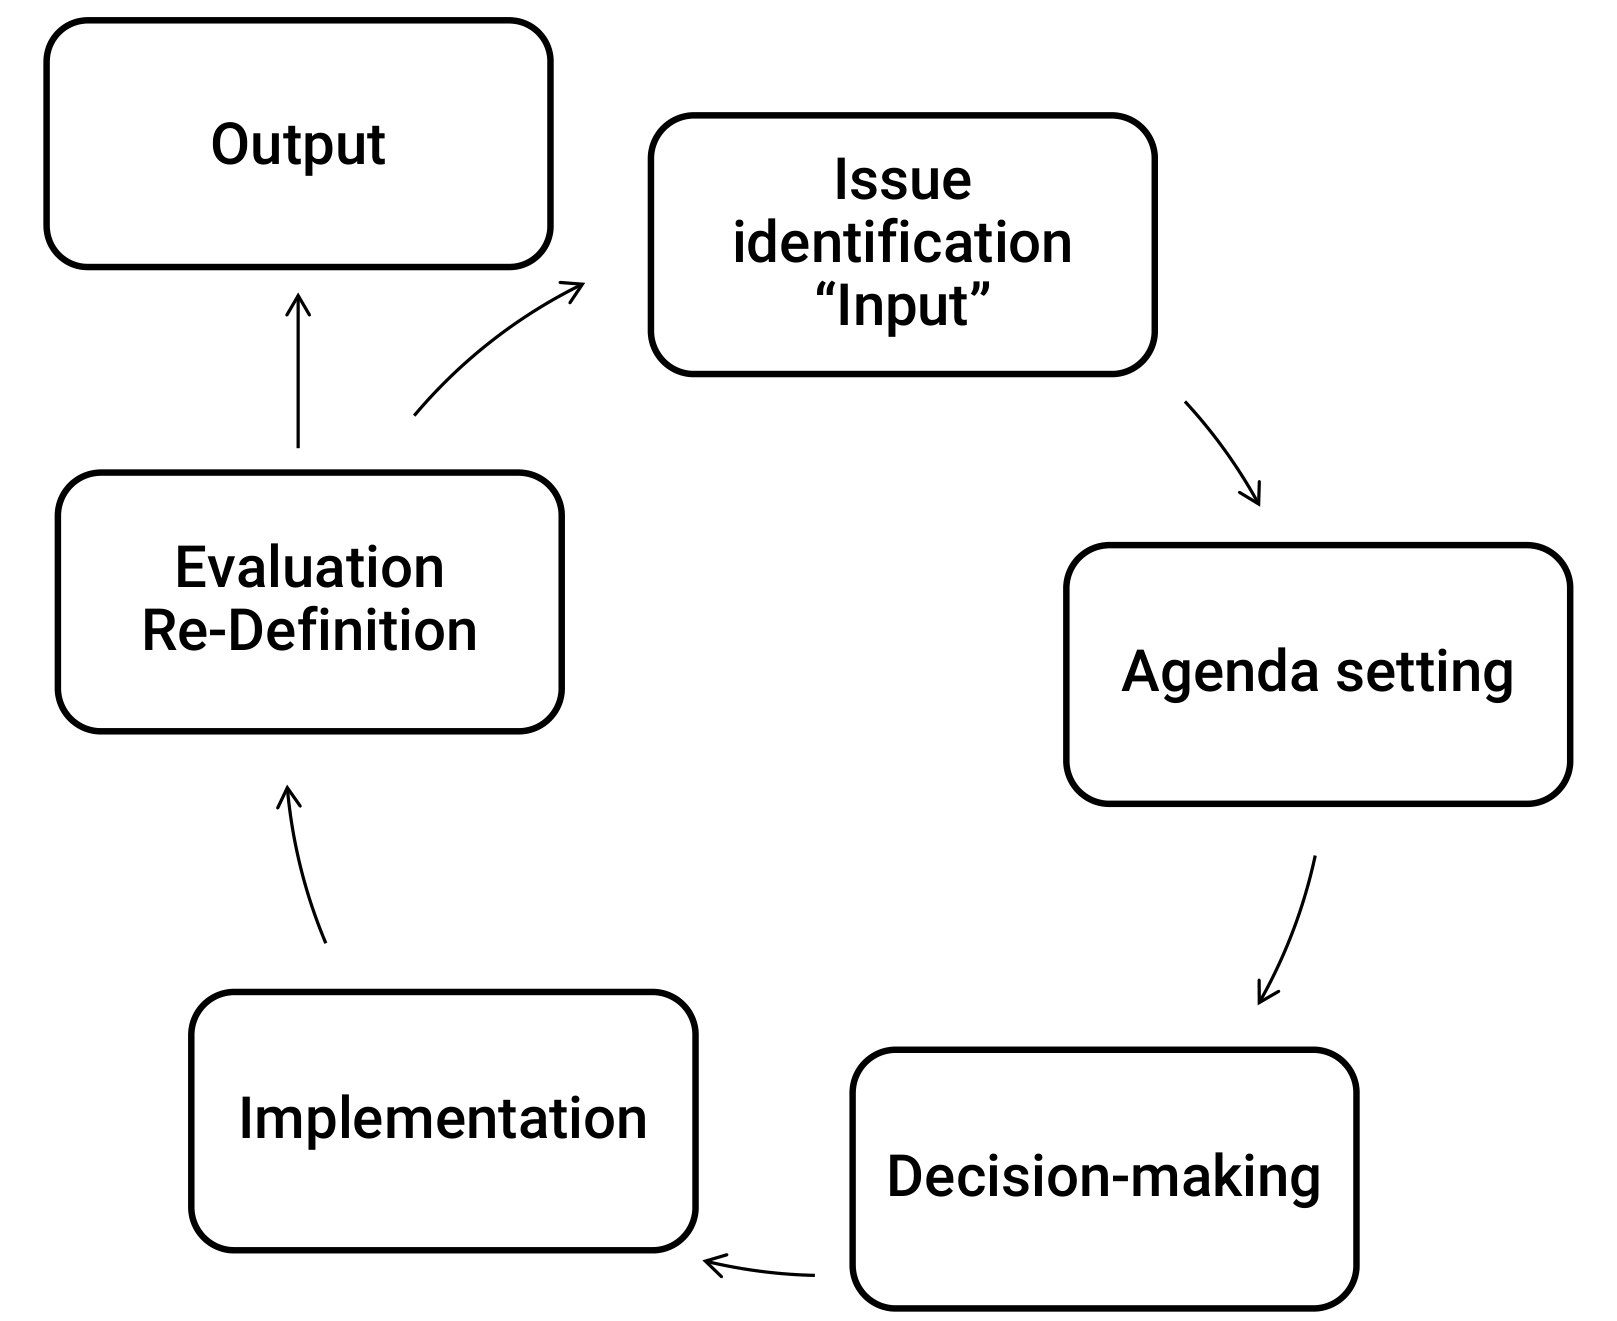
\includegraphics[width=0.6\linewidth]{img/national_decision_making}
	\caption{The decision making in Switzerland follows a so-called policy cycle}
	\label{fig:nationaldecisionmaking}
\end{figure}

\begin{table}[H]
	\begin{tabularx}{\linewidth}{c c}
		\cellcolor{DodgerBlue1!40} \textbf{Soft Instruments} & \cellcolor{DodgerBlue1!40} \textbf{Hard Instruments}\\
		 Education & Legal regulation \\
		 Support programs & Threshold values, bans \\
		 Information, awareness raising, advice & Economic coercion \\
		 Cooperation & Sanctions \\
		 Participation & Taxes, fees \\
		 Self-commitment & Certifications
	\end{tabularx}
	\caption{Instruments of Environmental and Sustainability Policy}
\end{table}

\begin{itemize}[nosep]
	\item \textbf{Absolute Poverty}
	\begin{itemize}
		\item Based on assumed minimal needs
		\item Household income is insufficient to afford basic necessities of life (food, shelter, housing)
		\item International poverty line: USD 1.90 a day
		\item Does not change by economic growth (USD 1.25 a day in 2005 prices)
		\item Possible to compare between countries and over time
	\end{itemize}
	\item \textbf{Relative Poverty}
	\begin{itemize}
		\item Based on income distribution
		\item Household income is a certain percentage below median incomes
		\item Household members cannot afford to actively participate in social activities that most people in a given country take for granted
		\item European standard concept of relative poverty: cut-off point - 60\% of median equalized disposable income
		\item Changes with economic growth
	\end{itemize}
\end{itemize}

\begin{figure}[H]
	\centering
	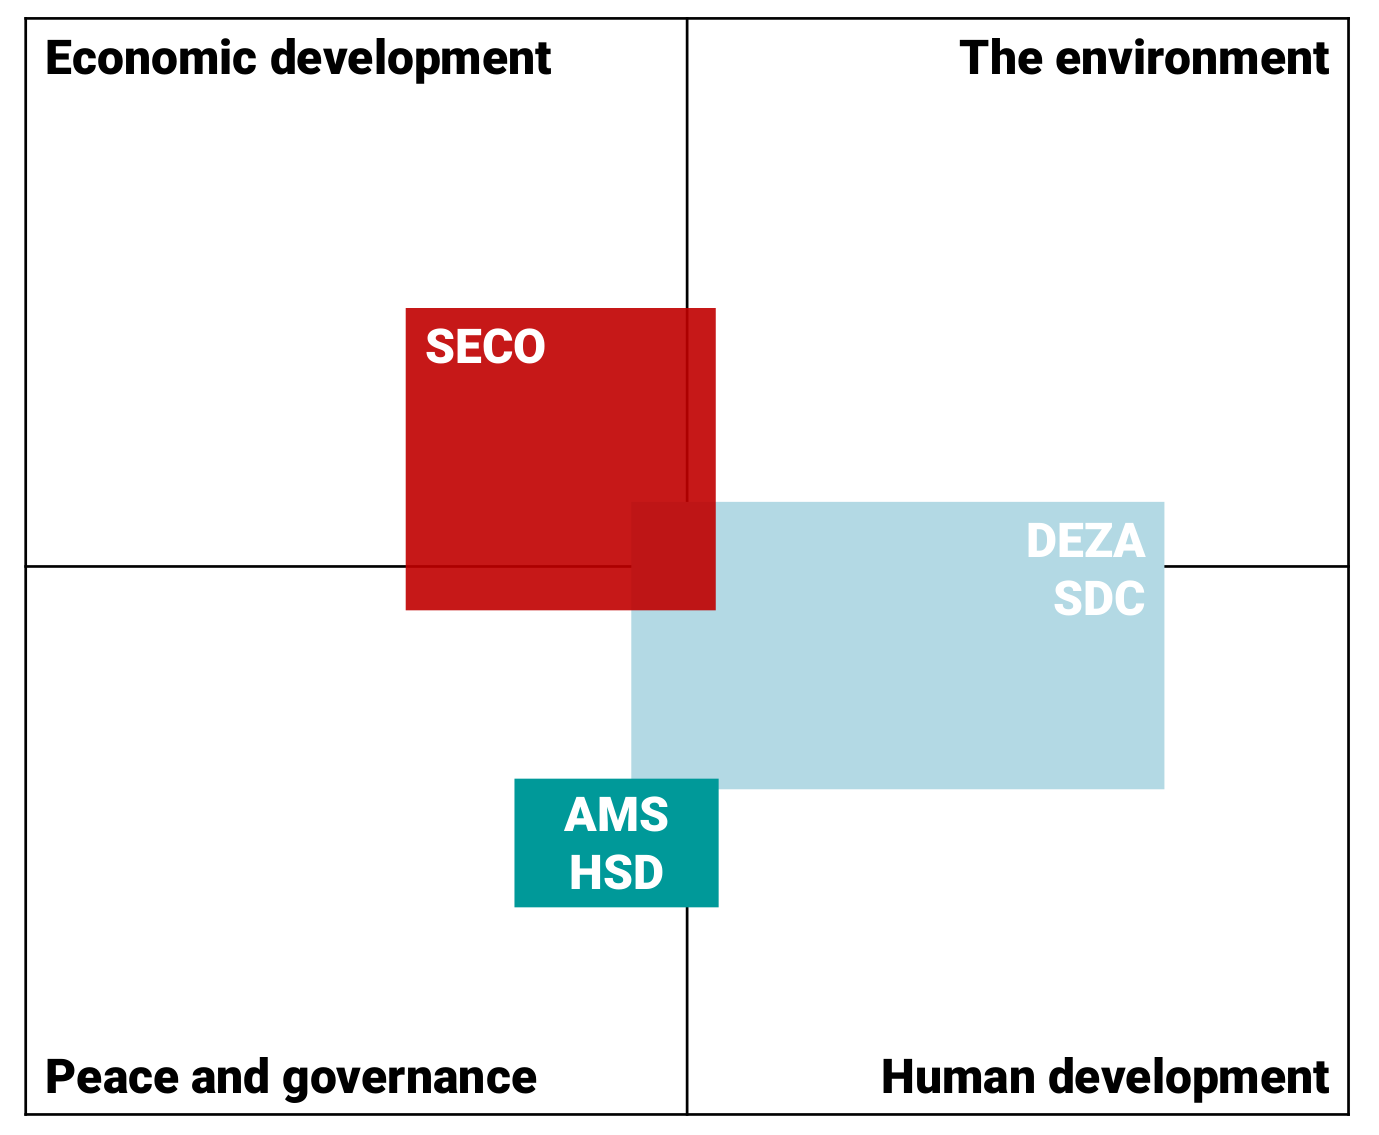
\includegraphics[width=0.6\linewidth]{img/swiss_development_coalition}
	\caption{Swiss bureaus working on economy development}
	\label{fig:swissdevelopmentcoalition}
\end{figure}

\begin{figure}[H]
	\centering
	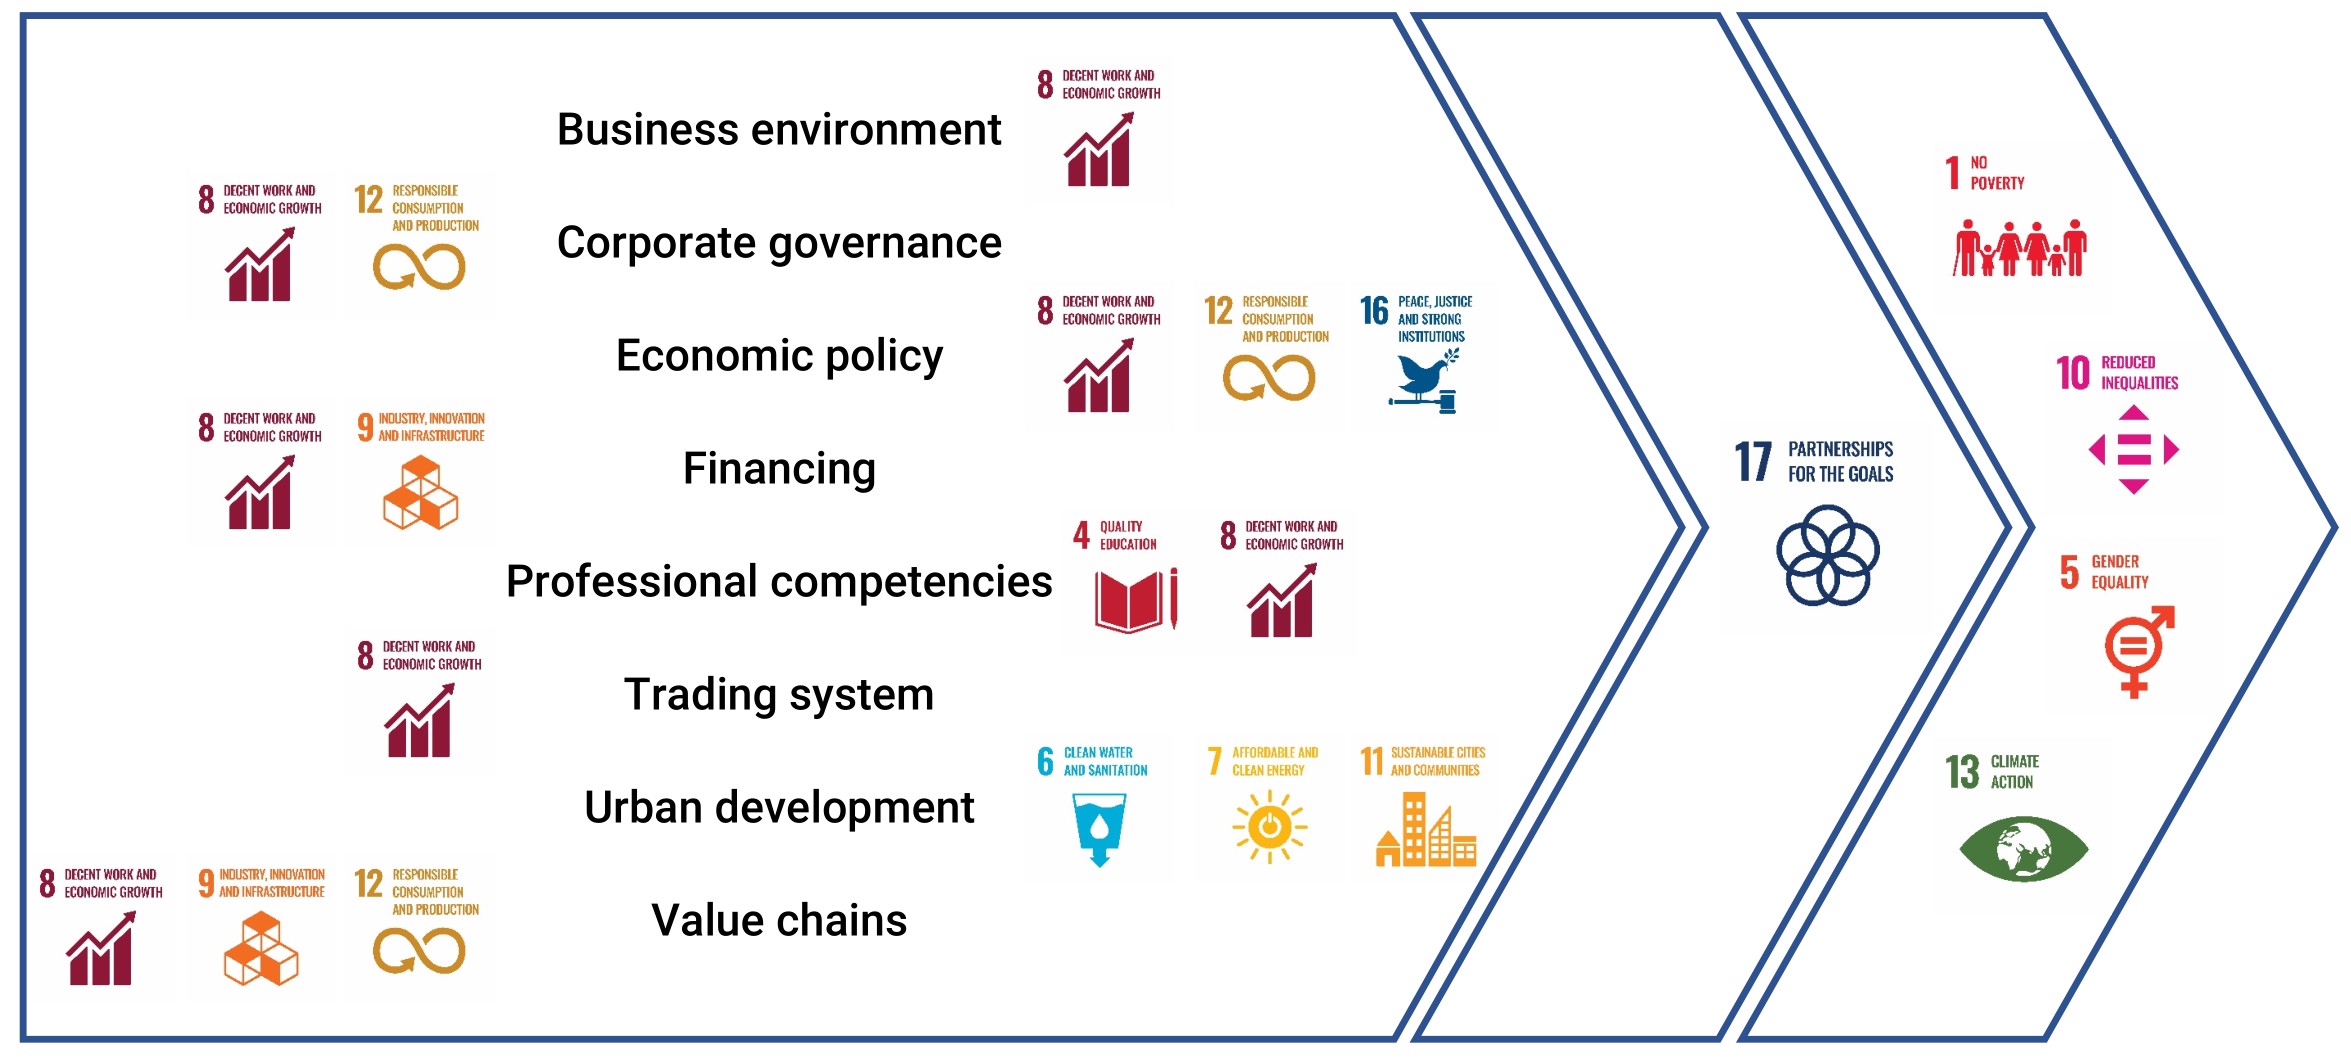
\includegraphics[width=0.8\linewidth]{img/SDG_targets_SECO.png}
	\caption{SDGs targeted by the SECO and developed in cooperation with international partners}
	\label{fig:secosdgtargets}
\end{figure}

\begin{figure}[H]
	\centering
	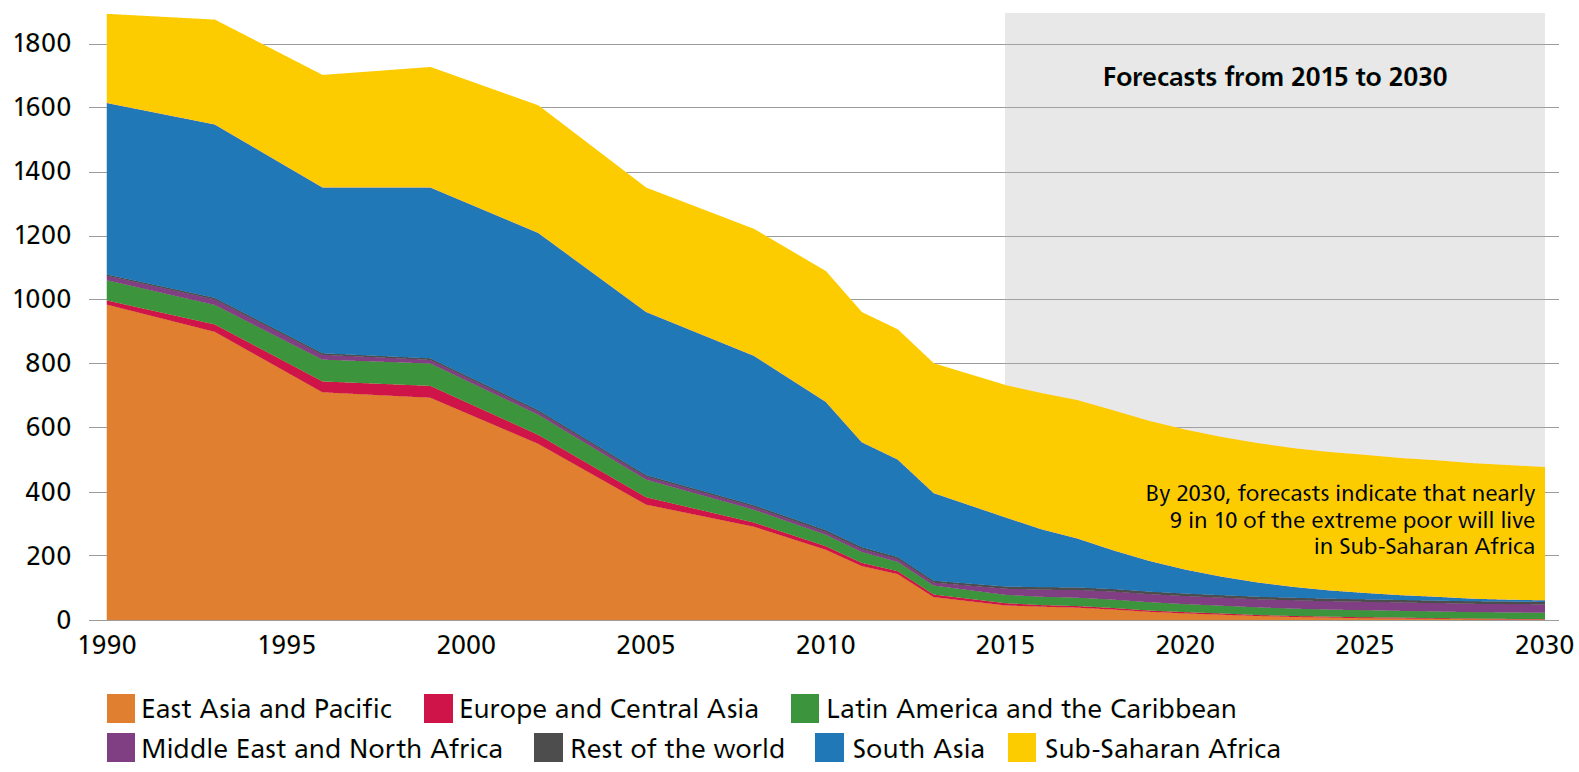
\includegraphics[width=0.8\linewidth]{img/people_living_extreme_poverty}
	\caption{Development of people living in extreme poverty}
	\label{fig:peoplelivingextremepoverty}
\end{figure}

\subsection{Swiss Green Economy Action Plan}
\begin{itemize}
	\item Six areas contributing towards a green economy
	\begin{itemize}
		\item Clean Technologies Master Plan
		\item Resource-efficient information and communication technologies
		\item Improving information on the environmental impact of products
		\item Greening the tax system (making environmental-friendly products having an advantage in the tax system)
		\item Comprehensive welfare measurement (common indicator is Gross Domestic Product (GDP), but GDP is growth based, and not necessarily reflects population health and welfare)
		\item Resource efficiency and sustainability in legislative drafts
	\end{itemize}
	\item Priority areas of the action plan
	\begin{itemize}
		\item Consumption and production (improve efficiency)
		\item Using fewer raw materials and produce less waste
		\item Cross-cutting instruments
		\item Set targets, monitor measures, prepare reports
	\end{itemize}
\end{itemize}

\subsection{Swiss Long-Term Climate Strategy}
\begin{itemize}
	\item Adopted on January 27, 2021
	\item Ties in with the revised $\text{CO}_2$ Act
	\item Obligation under the Paris Agreement
	\item 50\%-reduction in greenhouse gases by 2030
	\item Net-zero greenhouse emissions by 2050
	\item Difficult-to-avoid emissions should be offset by carbon capture and storage (CCS) or by negative emissions technologies (NETs)
	\item Ten basic strategic principles that will shape Swiss climate policy in the coming years
	\item Setting strategic targets for buildings, industry, transport, agricultural and food sectors, financial markets, aviation and the waste industry
\end{itemize}

\subsubsection{Ten Strategic Principles for Swiss Climate Policy}
These principles will shape the national and international policy of Switzerland in the coming years
\begin{enumerate}
	\item Switzerland will take advantage of the opportunities presented by a systematic transition to net zero
	\item Switzerland will assume its climate policy responsibility
	\item Priority will be given to reducing domestic emissions
	\item Emissions will be reduced across entire value chains
	\item All energy sources will be used effectively taking account of their optimal usage potential
	\item The Swiss Confederation and the cantons will gear their planning activities to net zero in all climate relevant areas
	\item The transition to net zero will be carried out in a socially acceptable way
	\item The transition to net zero will be achieved in an economically viable way
	\item The transition to net zero will also improve environmental quality
	\item The Long-Term Climate Strategy is based on openness to all types of technology
\end{enumerate}

\begin{figure}[H]
	\centering
	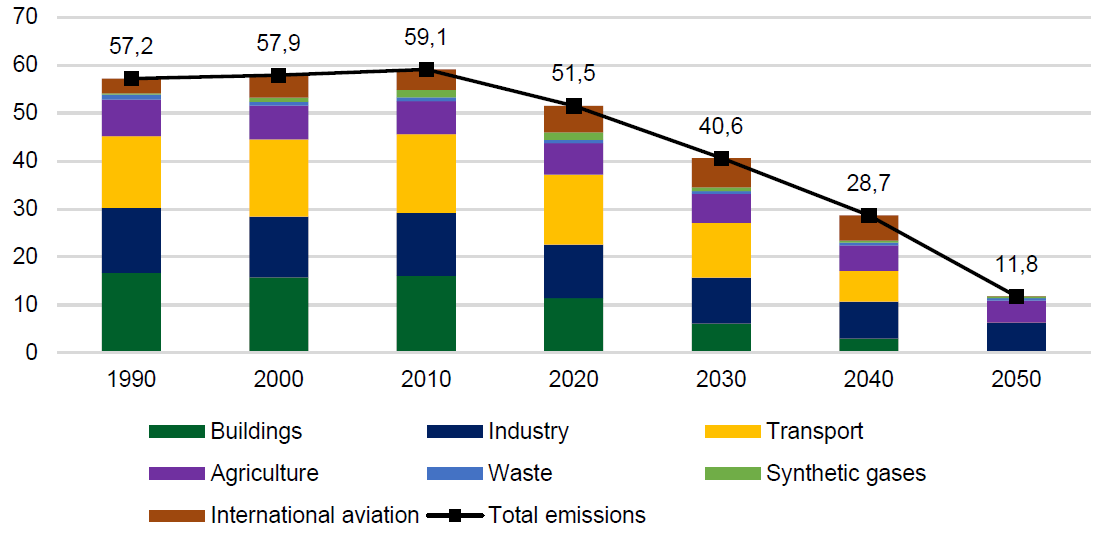
\includegraphics[width=0.8\linewidth]{img/development_emissions_plan_switzerland}
	\caption{Development of emissions by 2050 by sectors in tonnes of $\text{CO}_2$-equivalents according to a zero emissions basis scenario of EP2050+, including international aviation.}
	\label{fig:developmentemissionsplanswitzerland}
\end{figure}

\begin{figure}[H]
	\centering
	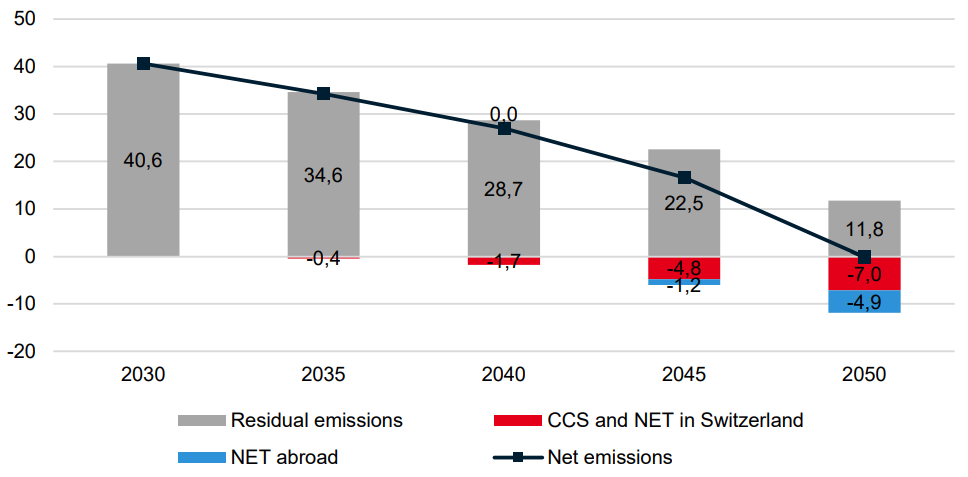
\includegraphics[width=0.8\linewidth]{img/development_remaining_emissions_plan_switzerland}
	\caption{Development of remaining emissions and contributions of negative emissions technologies (NET) and carbon capture and storage (CCS) in Switzerland and abroad according to the zero emissions basis scenario of EP2050+, including international aviation.}
	\label{fig:developmentremainingemissionsplanswitzerland}
\end{figure}

\subsubsection{Swiss National Action Plan on Business and Human Rights}
\begin{itemize}
	\item The UN Guiding Principles on Business and Human Rights sets out States' obligations and corporate responsibility regarding the impact of business activities on human rights
	\item The Federal Council is committed to prevent, mitigate and remediate business-related human rights abuse.
	\item Priority Actions
	\begin{itemize}
		\item Communication, that is the expectation of the federal government from corporations
		\item Support for business enterprises, mainly in the form of guidance for businesses, exchange of information, and development of expertise at Swiss embassies
		\item Policy coherence, meaning the improvement of interdepartmental cooperation
	\end{itemize}
\end{itemize}

\subsubsection{Swiss Anti-Corruption Strategy}
\begin{itemize}
	\item Approved on 25 November 2020
	\item Strategy's objectives
	\begin{itemize}
		\item Preventing and prosecuting cases of corruption
		\item Detection and repression
		\item International cooperation in the field of corruption
	\end{itemize}
	\item Anti-corruption obligations at international level
\end{itemize}

\subsubsection{Typology of NGOs}
\begin{tabularx}{\linewidth}{r r |c|c|}
	\multirow{4}{*}{\large\textbf{Beneficiary}} & \multirow{2}{*}{\textbf{Self}} & Alcoholics Anonymous & Labour Unions\\
	& & Chess Clubs & Trade Associations\\
	\cline{2-4}
	& \multirow{2}{*}{\textbf{Others}} & Salvation Army & WWF\\
	& & CARE & Amnesty International\\
	\cline{2-4}
	& & \textbf{Service} & \textbf{Advocacy}\\
	\multicolumn{2}{c}{} & \multicolumn{2}{c}{\large \textbf{Type of Activity}}
\end{tabularx}
\begin{itemize}
	\item Operational NGOs
	\item Advocacy NGOs
	\begin{itemize}
		\item Policy analysis and lobbying
		\item Impact upon government policy-making
		\item Advocacy Targets
		\begin{itemize}
			\item National\\
			Governments, corporations, other
			\item International
			\item Intergovernmental organizations, transnational corporations
		\end{itemize}
		\item Advocacy Strategy
		\begin{itemize}
			\item Collaborative\\
			Research, Education, Persuasion
			\item Adversarial\\
			Public Pressure, Litigation, Contestation
		\end{itemize}
	\end{itemize}
\end{itemize}

\begin{figure}[H]
	\centering
	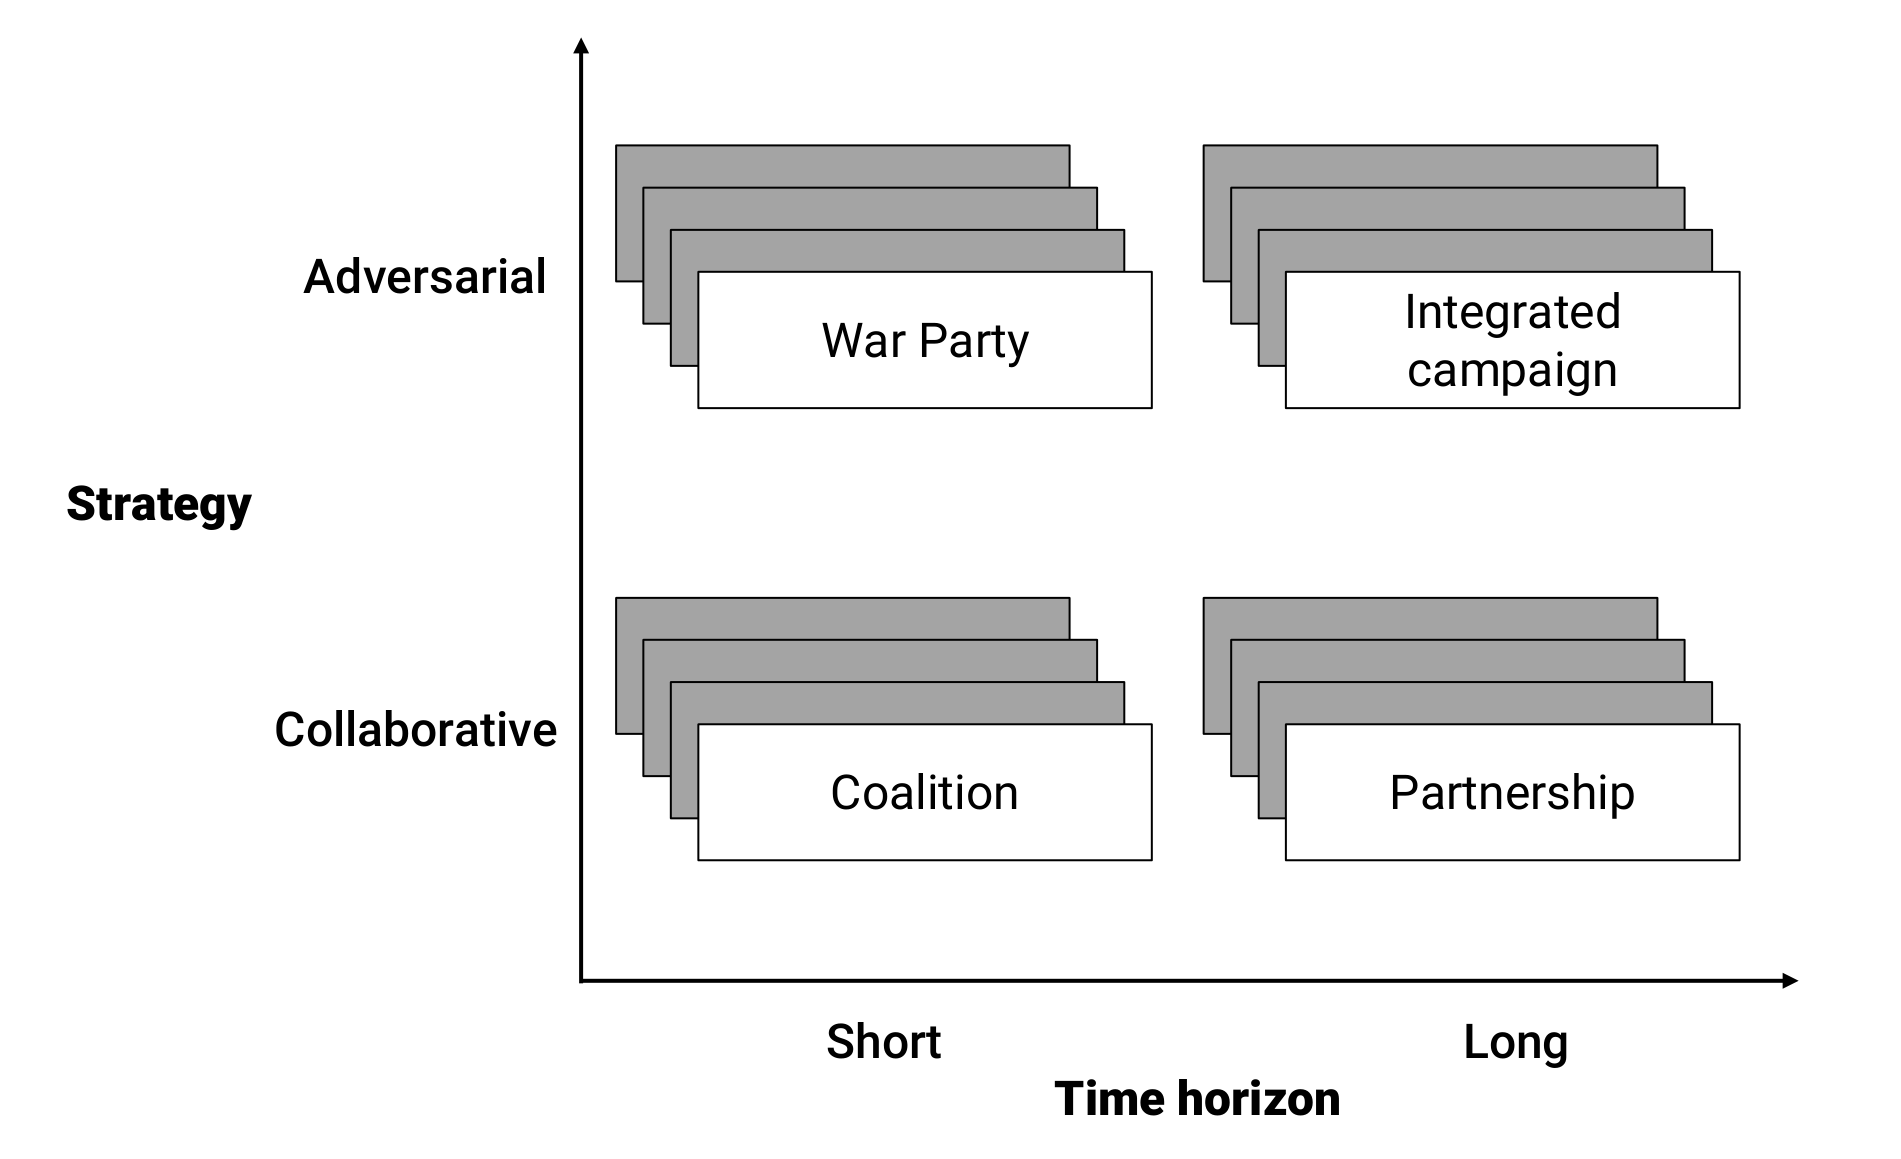
\includegraphics[width=0.8\linewidth]{img/ngo_campaign_architecture}
	\caption{NGO Campaign Architectures: Strategy, Time Horizon and Levels or Countries}
	\label{fig:ngocampaignarchitecture}
\end{figure}

\paragraph{Collaborative Strategies}
\begin{itemize}
	\item Short-term Coalitions:\\
	Mobilize affiliates and allies to shape policy outcomes
	\item Longer term Partnerships:\\
	Join forces with key actors to support ongoing policy change and implementation
\end{itemize}

\paragraph{Adversarial Strategies}
\begin{itemize}
	\item Short-term adversarial campaigns:\\
	Create public pressure, respond quickly to opportunities or threats
	\begin{itemize}
		\item Embarrass powerful actors
		\item Generate wide public visibility
	\end{itemize}
	\item Longer term initiatives:\\
	Mobilize and coordinate resources to sustain multi-year campaigns to change policies and monitor implementation
\end{itemize}

% TODO Check if formatting is still ok
\clearpage
\subsubsection{Goals, Targets and Tactics of NGOs}
\begin{tabularx}{\linewidth}{l p{0.25\linewidth} p{0.25\linewidth} p{0.25\linewidth}}
	\cellcolor{DodgerBlue1!40} & \cellcolor{DodgerBlue1!40} \textbf{Mainstream} & \cellcolor{DodgerBlue1!40} \textbf{Moderate} & \cellcolor{DodgerBlue1!40} \textbf{Radical}\\
	\textbf{Goals} & Enforcement of existing laws and norms & Small change to institutions/ laws or their interpretation & Major change to central tenants of dominant institutions \\
	\textbf{Targets} & Law Violators & "Bad Boys" representing the "worst" of the dominant institutions & Symbols of dominant institutions\\
	\textbf{Tactics} & \begin{itemize}[
			left=0pt,
			nosep,
			before={\begin{minipage}[t]{\hsize}},
			after={\end{minipage}}
		]
		\item Use of dominant institutions of enforcement
		\item Less emotional, more rational appeal
	\end{itemize} & \begin{itemize}[
		left=0pt,
		nosep,
		before={\begin{minipage}[t]{\hsize}},
		after={\end{minipage}}
	]
		\item Use of dominant institutions that define and refine the laws and norms
		\item  Appeal to public opinion
	\end{itemize} & \begin{itemize}[
	left=0pt,
	nosep,
	before={\begin{minipage}[t]{\hsize}},
		after={\end{minipage}}
	]
		\item Counter-institutional tactics attempting to reshape public opinion
		\item Appeal to Emotions
\end{itemize}
\end{tabularx}
\begin{figure}[H]
	\centering
	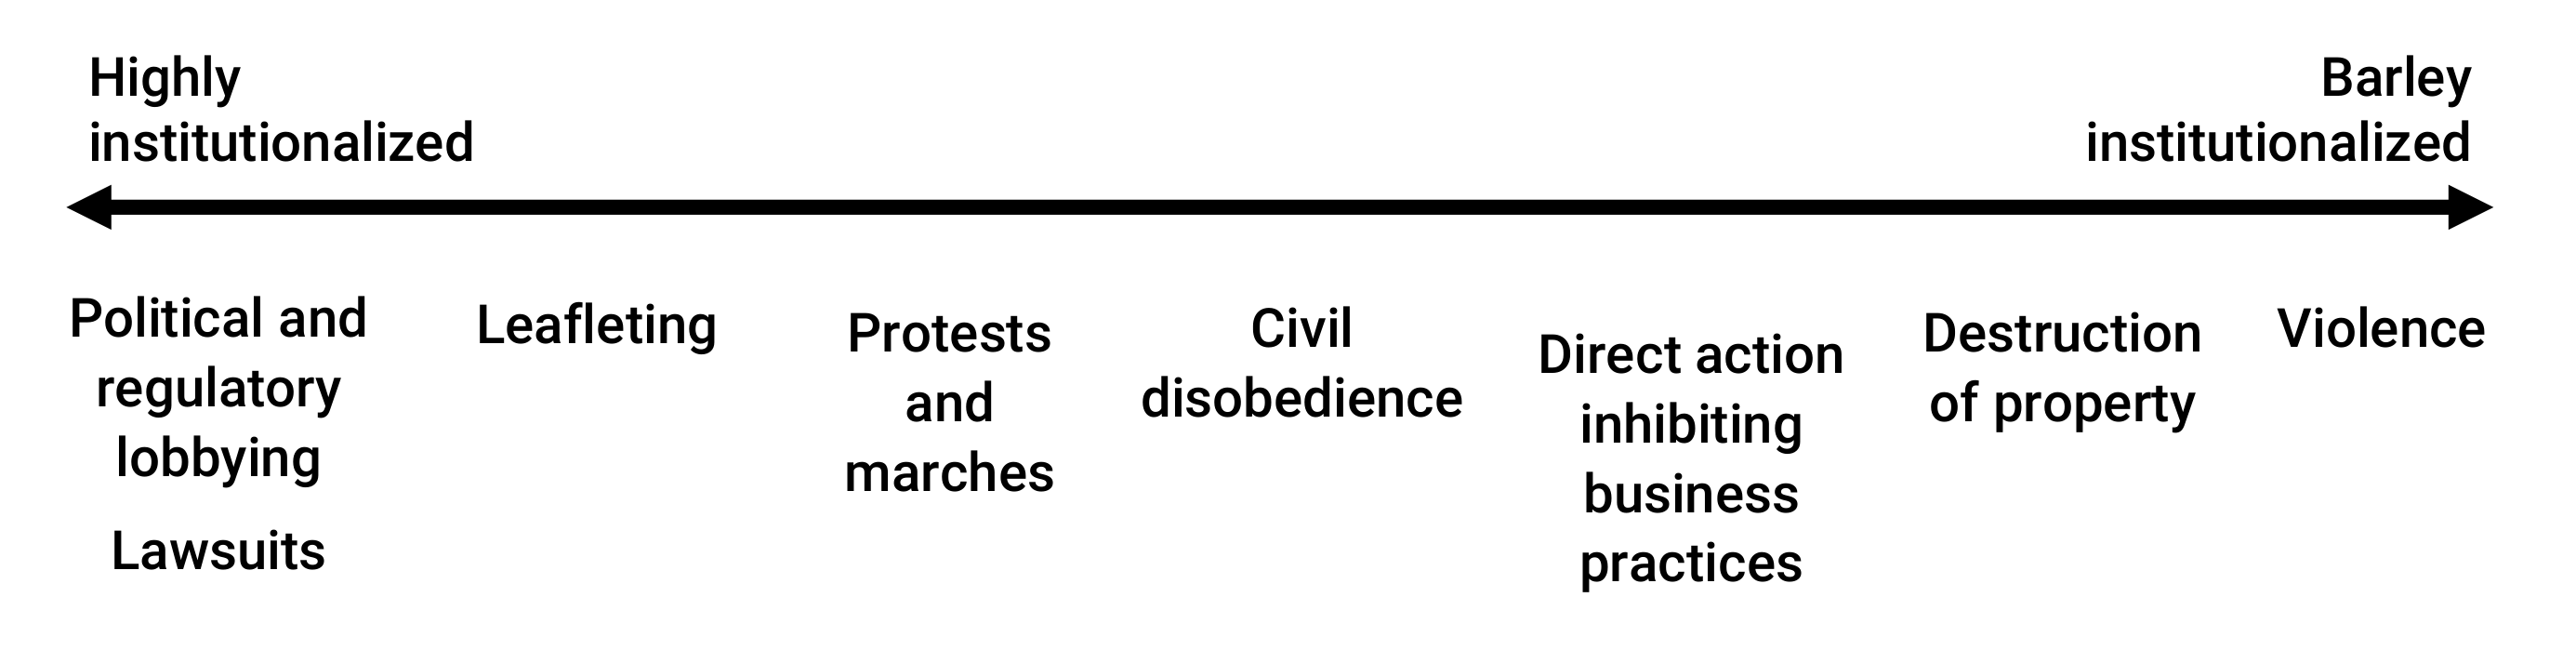
\includegraphics[width=0.8\linewidth]{img/ngo_tactics}
	\caption{Tactics employed by NGOs}
	\label{fig:ngotactics}
\end{figure}

\subsection{Organisational Response to Environmental Demands}

\begin{quote}
	\textquotedblleft There is one and \textbf{only one social responsibility of business} -- to use its resources and engage in \textbf{activities designed to increase its profits} so long as it \textbf{stays within the rules of the game}, which is to say, engages in open and free competition \textbf{without deception or fraud}.\textquotedblright\\
	\hspace*{1em} - Milton Friedman
\end{quote}

\begin{table}[H]
	\footnotesize
	\begin{tabularx}{\linewidth}{p{0.1\linewidth} p{0.25\linewidth} p{0.25\linewidth} p{0.25\linewidth}}
		\cellcolor{SteelBlue1!75} & \cellcolor{SteelBlue1!75} \textbf{Coercive Isomorphism} & \cellcolor{SteelBlue1!75} \textbf{Mimetic Isomorphism} & \cellcolor{SteelBlue1!75} \textbf{Normative Isomorphism}\\
		\textbf{Results from} & \begin{itemize}[
				left=0pt,
				nosep,
				before={\begin{minipage}[t]{\hsize}},
				after={\end{minipage}}
			]
			\item Resource dependency
			\item Formal and informal pressure
			\item Government mandate
			\item Cultural expectations in the society
			\item Monitoring and sanctioning of wrongdoers
		\end{itemize} & \begin{itemize}[
				left=0pt,
				nosep,
				before={\begin{minipage}[t]{\hsize}},
				after={\end{minipage}}
			]
			\item Environmental uncertainty
			\item Ambiguous goals, unclear solutions
			\item Intentionally through consulting firms or industry trade associations
			\item Unintentionally through employee transfer or turnover
		\end{itemize} & \begin{itemize}[
				left=0pt,
				nosep,
				before={\begin{minipage}[t]{\hsize}},
				after={\end{minipage}}
			]
			\item Professionalisation through formal education
			\item Professional networks
			\item Filtering of personnel through recruitment and promotion practices
		\end{itemize}
	\end{tabularx}
	\caption{The neo-institutional perspective}
\end{table}

\begin{table}[H]
	\footnotesize
	\begin{tabularx}{\linewidth}{p{0.1\linewidth} p{0.25\linewidth} p{0.25\linewidth} p{0.25\linewidth}}
		\cellcolor{SteelBlue1!75} & \cellcolor{SteelBlue1!75} \textbf{Coercive Isomorphism} & \cellcolor{SteelBlue1!75} \textbf{Mimetic Isomorphism} & \cellcolor{SteelBlue1!75} \textbf{Normative Isomorphism}\\
		\textbf{Results from} & \begin{itemize}[
			left=0pt,
			nosep,
			before={\begin{minipage}[t]{\hsize}},
				after={\end{minipage}}
			]
			\item  Strategically manipulating external demands without adjusting organisational structures and practices
		\end{itemize} & \begin{itemize}[
			left=0pt,
			nosep,
			before={\begin{minipage}[t]{\hsize}},
				after={\end{minipage}}
			]
			\item Decoupling organizational responses from actual practices
			\item Symbolically but not substantially aligning organisational structures and practices to external demands
		\end{itemize} & \begin{itemize}[
			left=0pt,
			nosep,
			before={\begin{minipage}[t]{\hsize}},
				after={\end{minipage}}
			]
			\item Isomorphically changing organizational structures and practices to conform to external demands
			\item Two main avenues:
			\begin{itemize}[nosep, left=1em]
				\item proactive approach
				\item reactive approach
			\end{itemize}
		\end{itemize}
	\end{tabularx}
	\caption{The strategic choice perspective}
\end{table}

\begin{tabularx}{\linewidth}{l X}
	\textbf{Defensive} &  Deny practices, outcomes, or responsibilities\\
	\textbf{Compliance} & Adopt a policy-based compliance approach as a cost of doing business\\
	\textbf{Managerial} & Embed the societal issue in the core management processes\\
	\textbf{Strategic} & Integrate the societal issue into the core business strategies\\
	\textbf{Civil} & Promote broad industry participation in corporate responsibility
\end{tabularx}

\begin{figure}[H]
	\centering
	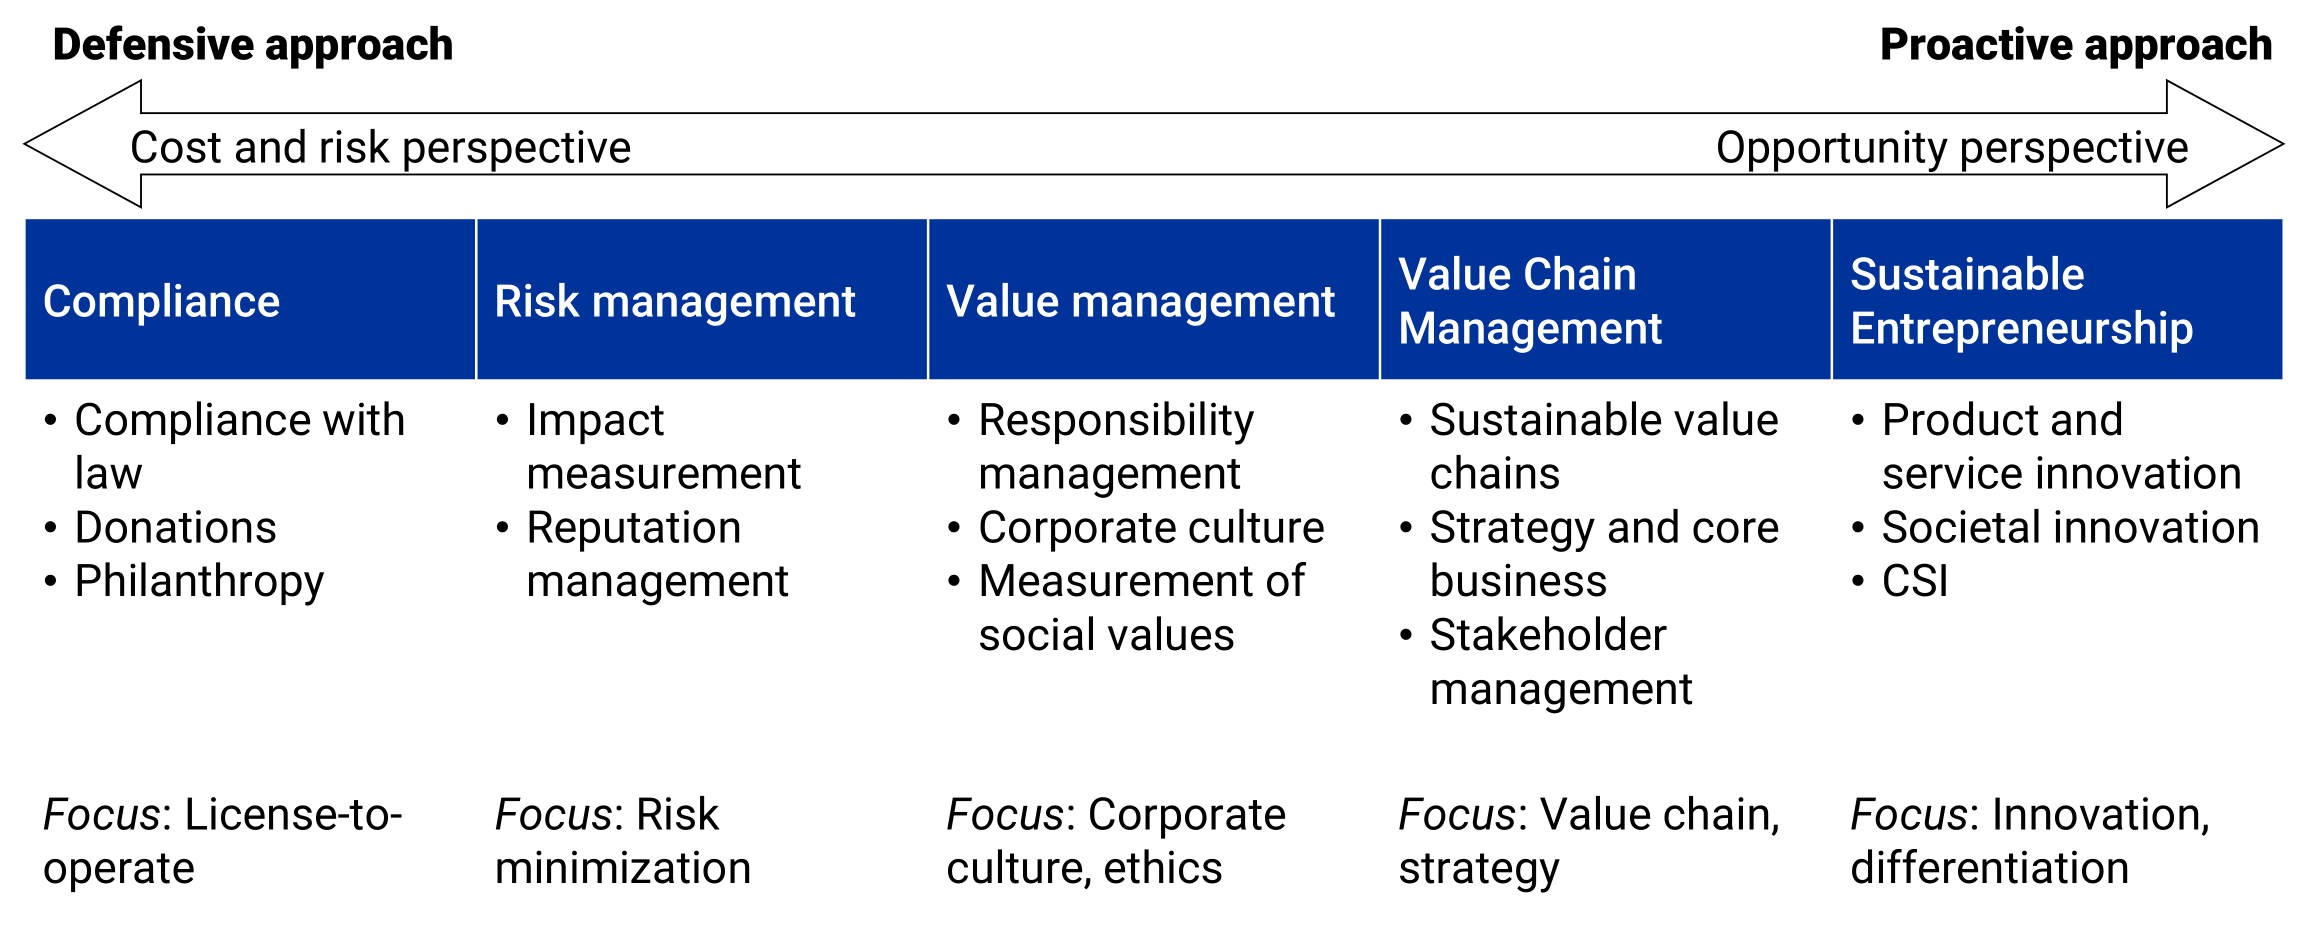
\includegraphics[width=0.9\linewidth]{img/organisational_approaches_environmental_demands}
	\caption{Different approaches and focii to respond to environmental demands as an organisation}
	\label{fig:organisationalapproachesenvironmentaldemands}
\end{figure}

\begin{figure}[H]
	\centering
	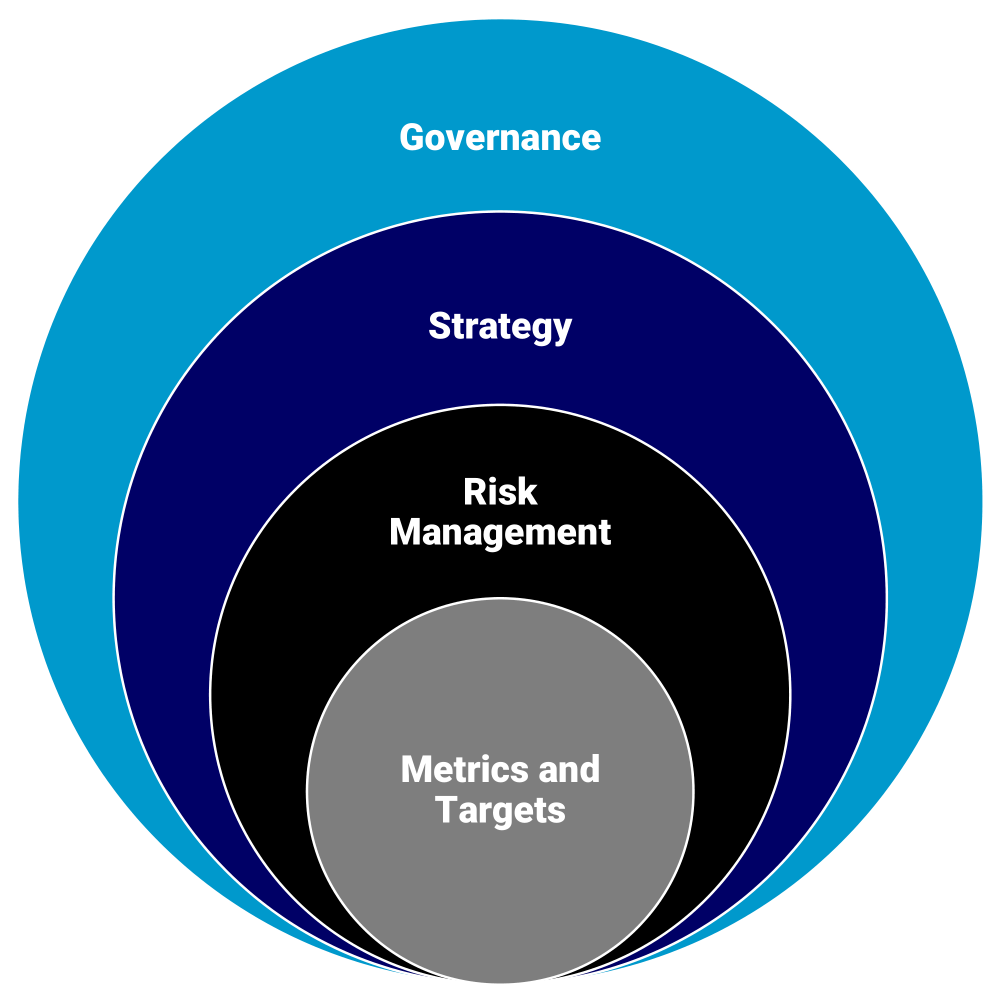
\includegraphics[width=0.4\linewidth]{img/core_elements_sustainability_management}
	\caption{Core elements of sustainability management processes}
	\label{fig:coreelementssustainabilitymanagement}
\end{figure}

\begin{itemize}[label=, left=0pt]
	\item \textbf{Governance}\\
	The organisation's governance around sustainability-related risks and opportunities
	\item \textbf{Strategy}\\
	The actual and potential impacts of sustainability-related risks and opportunities on the organisation's businesses, strategy, and financial planning
	\item \textbf{Risk Management}\\
	The processes used by the organisation to identify, assess, and manage sustainability-related risks
	\item \textbf{Metrics and Targets}\\
	The metrics and targets used to assess and manage relevant sustainability-related risks and opportunities
\end{itemize}

\begin{figure}[H]
	\centering
	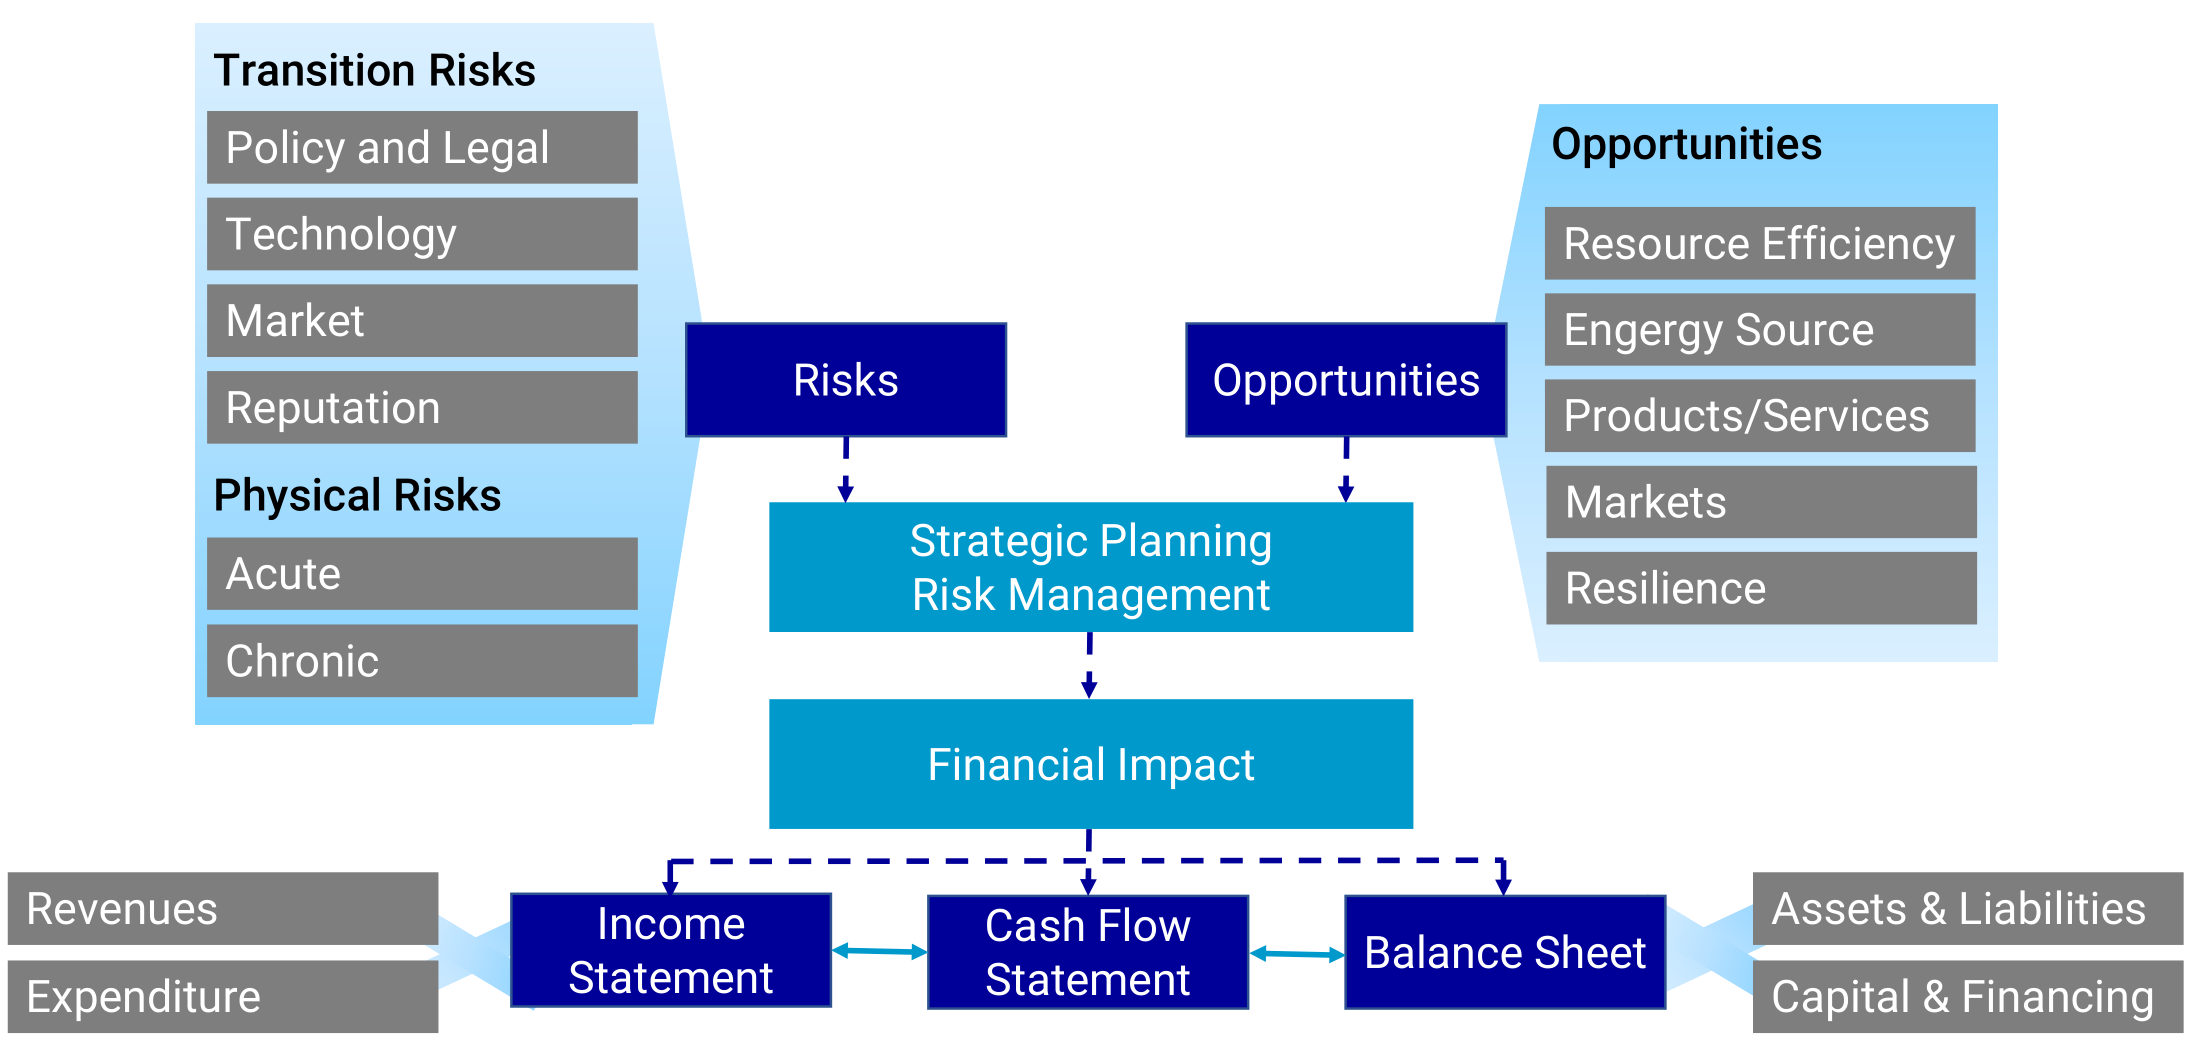
\includegraphics[width=0.8\linewidth]{img/sustainability_risks_opportunities_impact}
	\caption{Sustainability-related risks, opportunities, and financial impact}
	\label{fig:sustainabilityrisksopportunitiesimpact}
\end{figure}

\begin{enumerate}
	\item[] \textbf{Principles for Effective Disclosures}
	\item Disclosures should represent relevant information
	\item Disclosures should be specific and complete
	\item Disclosures should be clear, balanced, and understandable
	\item Disclosures should be consistent over time
	\item Disclosures should be comparable among companies within a sector, industry, or portfolio
	\item Disclosures should be reliable, verifiable, and objective
	\item Disclosures should be provided on a timely basis
\end{enumerate}

\clearpage
\subsubsection{Ethics and Compliance Training}
Compliance training often has the complication of being opposed or lateral to business targets
\begin{tabularx}{\linewidth}{p{0.26\linewidth} p{0.26\linewidth}}
	\textbf{Business Targets} & \textbf{Compliance Targets}\\
	\hline
	\begin{itemize}[
		left=0pt,
		nosep,
		before={\begin{minipage}[t]{\hsize}},
			after={\end{minipage}}
		]
		\item Time
		\item Budget
		\item Quality
		\item Technology
	\end{itemize} & Coping adequately with
	\begin{itemize}[
		left=0pt,
		nosep,
		before={\begin{minipage}[t]{\hsize}},
			after={\end{minipage}}
		]
		\item Values
		\item Standards
		\item Laws
		\item Rules
		\item Regulations
		\item ...
	\end{itemize} 
\end{tabularx}

\subsection{Individuals Response to Environmental Demands}
\subsubsection{External and Internal Barriers to Behavioural Change}
\begin{center}
	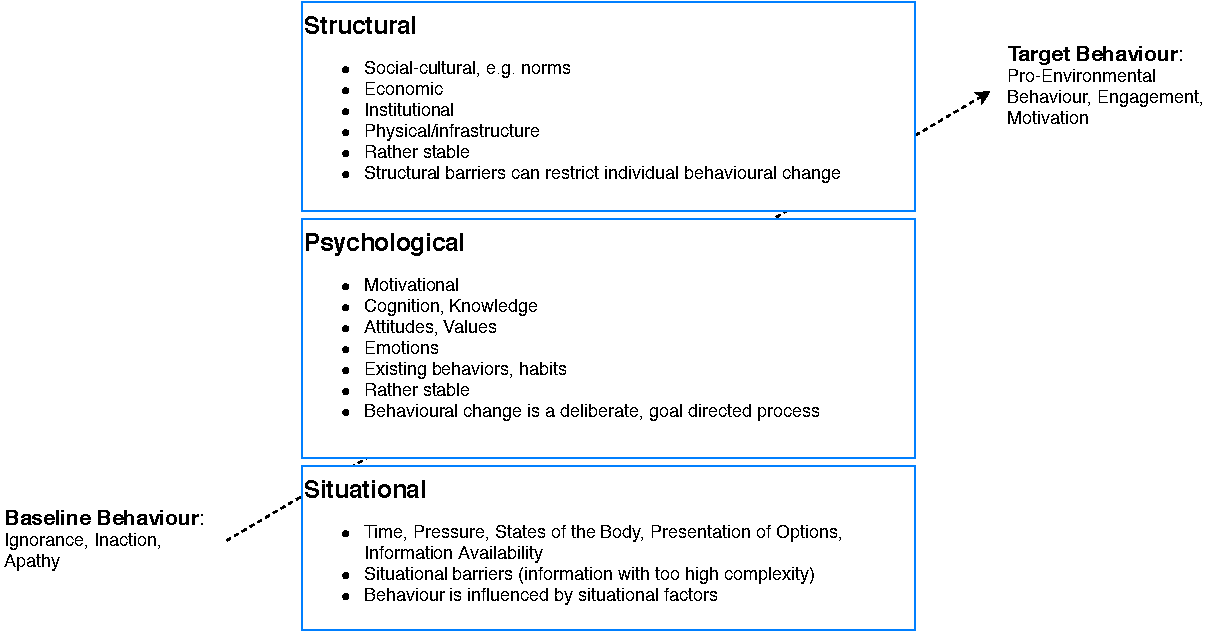
\includegraphics[width=0.9\linewidth]{img/behavioural_change}
\end{center}

\subsubsection{Habits and Biases}
\begin{itemize}
	\item Behaviour is highly habitual
	\item Habits: learned, highly automatized, stable behavioural patterns
	\item Approx. 35.53\% of our daily behaviours are habits (e.g., food choice, mobility, household)
	\item Habits help us save cognitive effort -- automatic and unconscious, based on situational cues
	\item To replace habitual behaviours, a lot of self-control (motivation) is needed (inhibit automatic response, focus on new behaviour), which is a limited resource
	\item Strong habits and biases can render norms and information ineffective
	\item People are biased towards the present
	\item Present bias: the tendency to over-value immediate rewards at the expense of long-term intentions (to protect the environment, save energy)
	\item Limited patience: People prefer to have the reward (convenience, comfort, social approval) now, and pay for it later; 'paying' for a delayed, uncertain reward is not a very attractive deal
\end{itemize}

\subsubsection{Four Component Model of Ethical Decision Making}
\begin{enumerate}
	\item \textbf{Awareness}
	\item \textbf{Judgement}
	\item \textbf{Motivation and Intention}
	\item \textbf{Ethical or Unethical Behaviour}
\end{enumerate}

\subsubsection{Factors That Promote Deviant Behaviour}
\begin{center}
	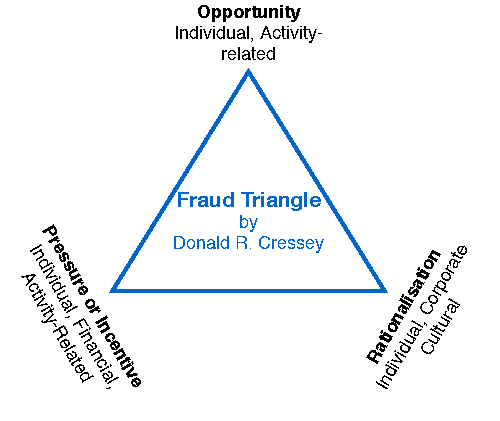
\includegraphics[width=0.5\linewidth]{img/fraud_triangle}
\end{center}

% TODO Write Intervention Strategies

\subsubsection{Nudging}
\begin{figure}[H]
	\centering
	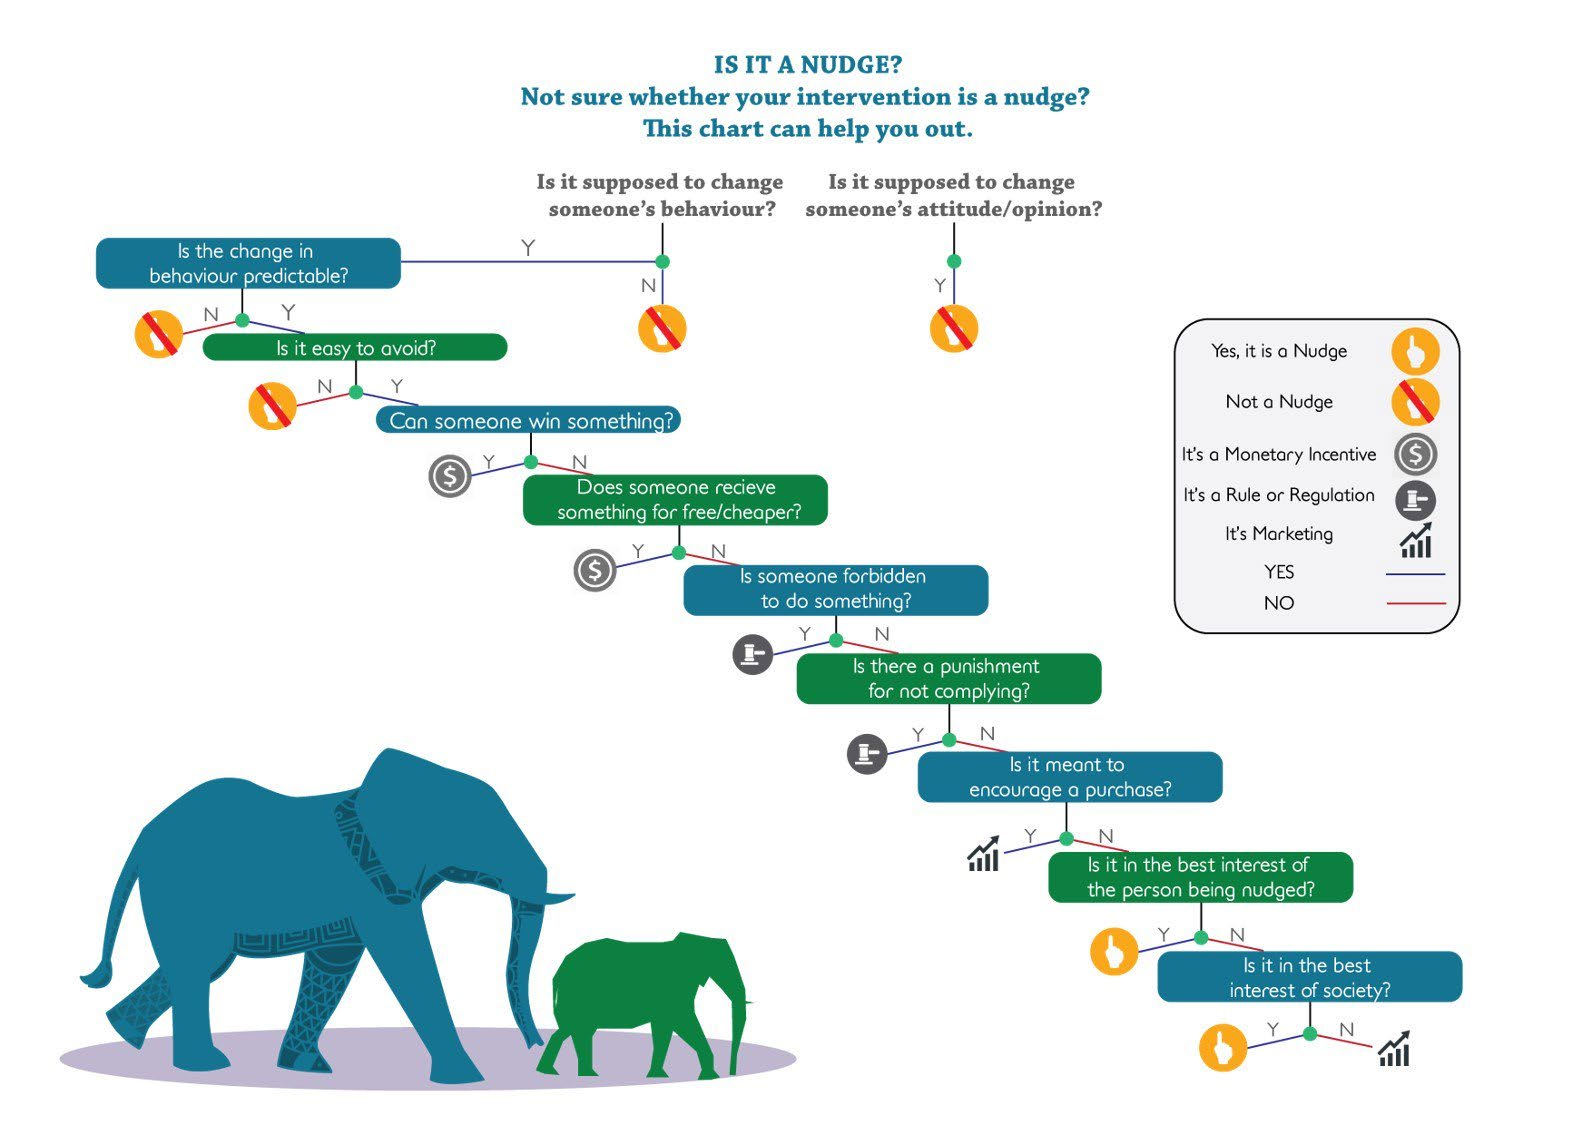
\includegraphics[width=0.7\linewidth]{img/nudging}
	\caption{\textquotedblleft Is it a nudge?\textquotedblright\ by Christina Gravert, 2017}
	\label{fig:nudging}
\end{figure}


\section{Life Cycle Thinking}

\begin{figure}[H]
	\centering
	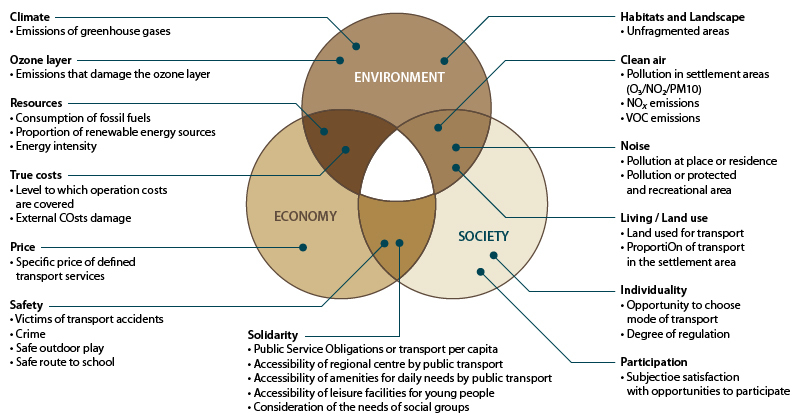
\includegraphics[width=0.8\linewidth]{img/three_modes_development.jpg}
	\caption{The Triple Bottom Line of Business with examples}
\end{figure}

\subsection{Life Cycle Sustainability Assessment}
The Life Cycle Sustainability Assessment integrates three aspects
\begin{itemize}
	\item Environmental (LCA or E-LCA)
	\item Social (S-LCA)
	\item Economic (Life Cycle Costs LCC)
\end{itemize}
\begin{equation*}
	\text{LCSA} = \text{LCA} + \text{SLCA} + \text{LCC}
\end{equation*}

\subsubsection{(Environmental) Life Cycle Assessment}
Systematic analysis of the environmental impacts of products throughout their entire life cycle, keyword 'cradle-to-grave'. This includes all environmental impacts during production, use phase, recycling or disposal of the product, as well as up- and downstream processes.

\paragraph{Motivation for LCA from a Corporate Perspective}
\begin{itemize}
	\item Product Analysis
	\item Product Development
	\item Product Comparison\\
	Compare different alternatives, performance in relation to competitors, selection of raw-materials, intermediate products, components and suppliers
\end{itemize}
\paragraph{Areas of Application}
\begin{itemize}
	\item Environmental Management\\
	Use environmentally friendly products, processes and sustainable procurement
	\item Product Marketing\\
	Leverage positive impression of sustainability benefits, have a basis for certification with an environmentally friendly label
	\item Legislation
\end{itemize}

\paragraph{How to Optimise Environmental Performance}
\begin{itemize}
	\item Have a comprehensive, holistic, environmental view
	\item Consider a large number of environmental impacts
	\item Consider the entire life cycle
	\item Should be suitable for Corporate Management Systems
	\item Quantify environmental impacts
	\item Be practical
\end{itemize}

\begin{figure}[H]
	\centering
	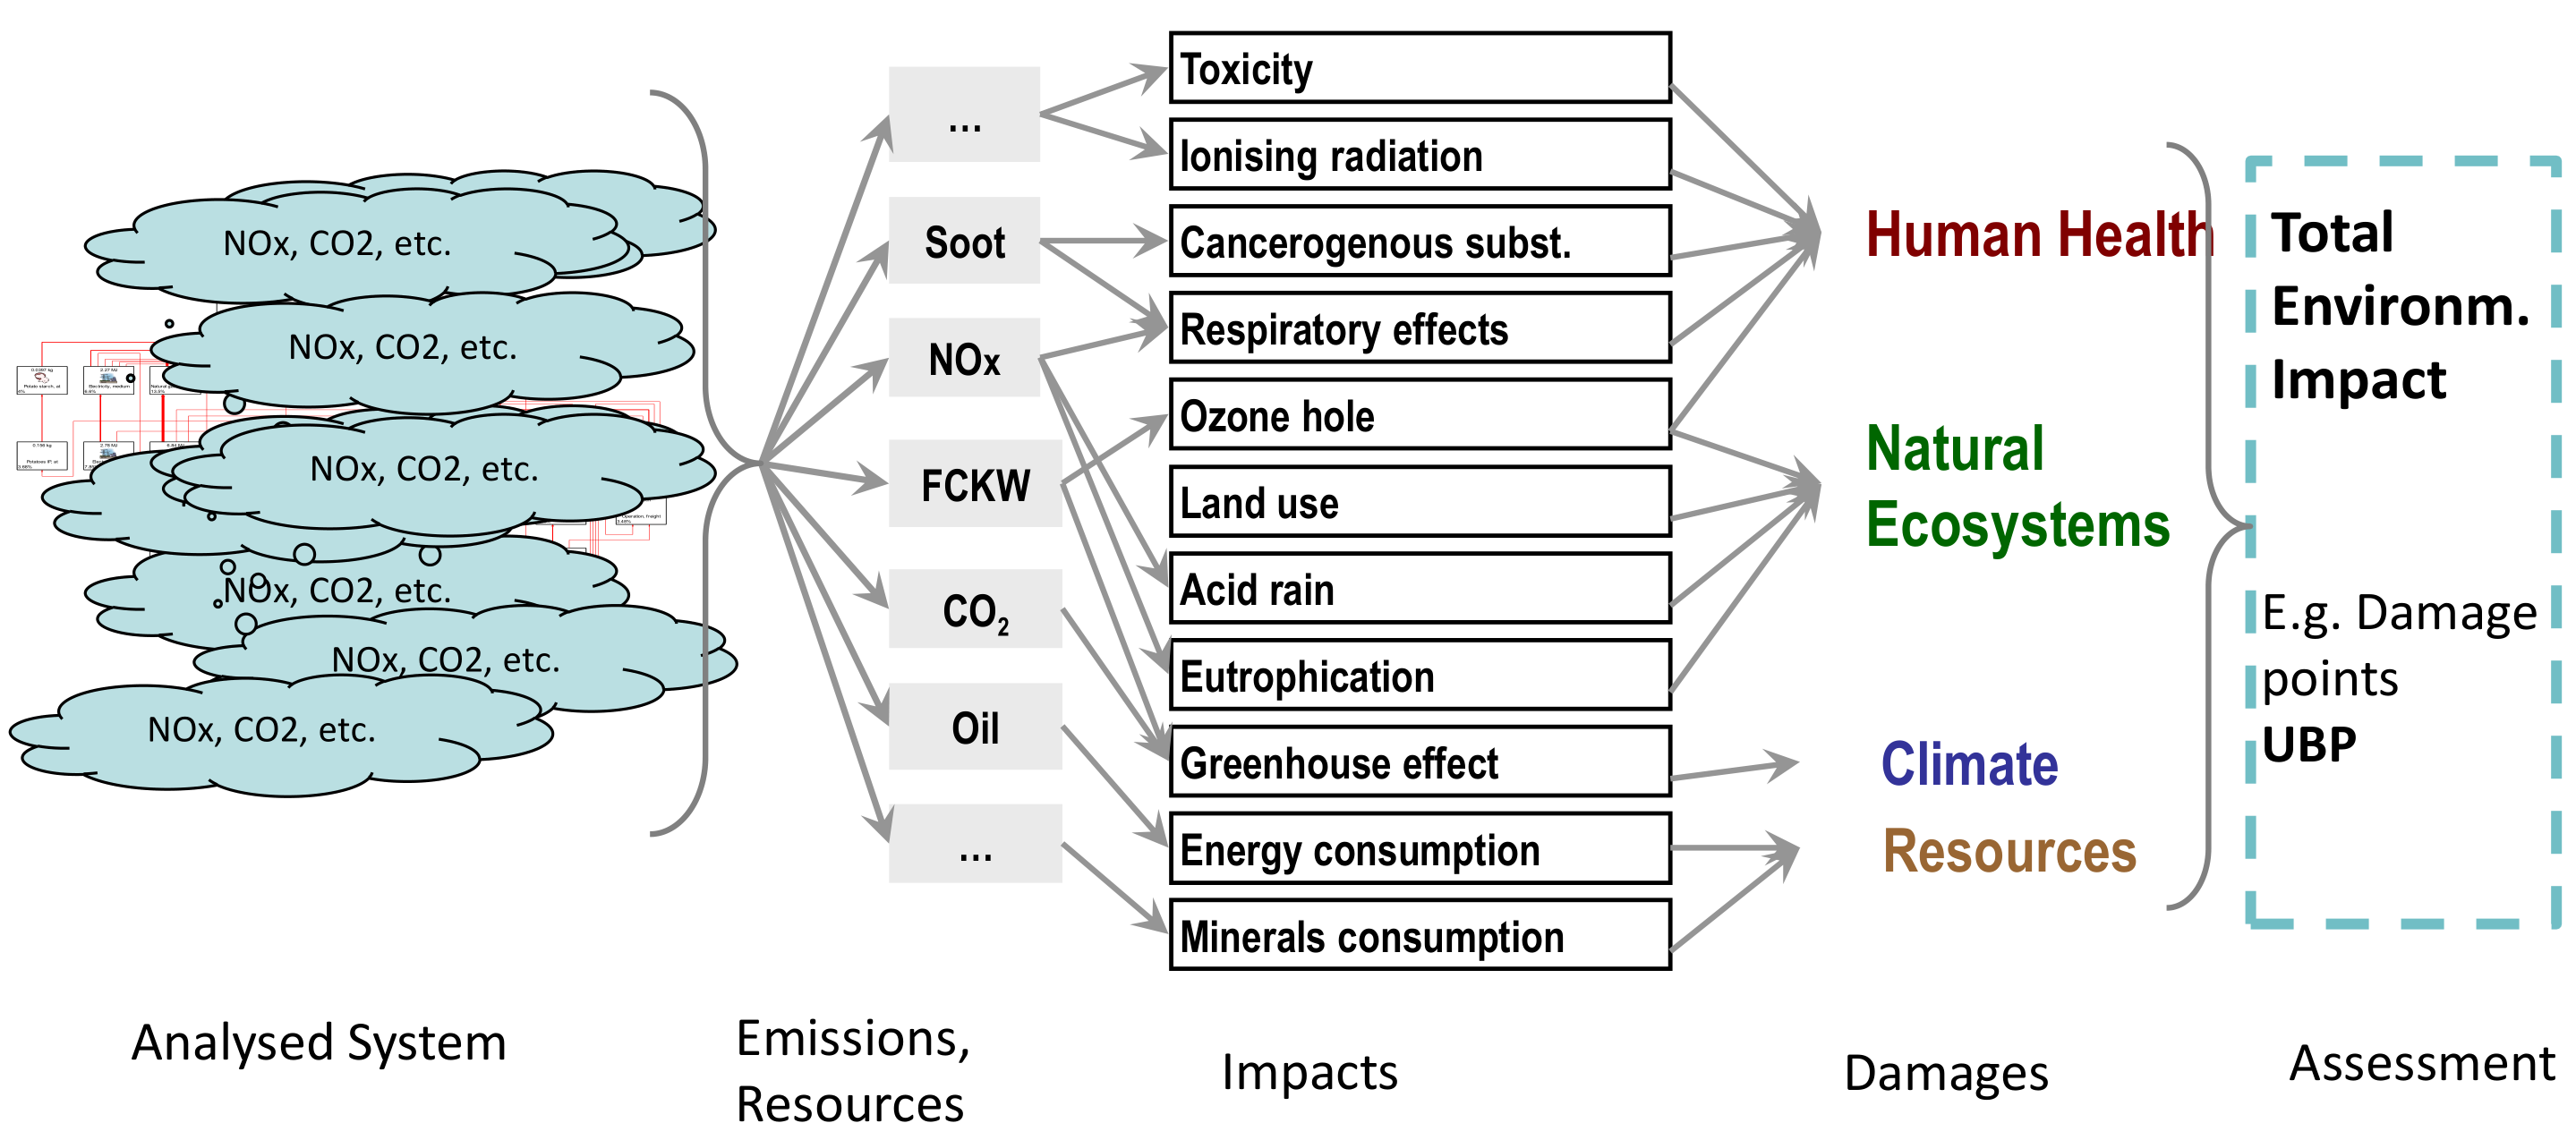
\includegraphics[width=0.8\linewidth]{img/life_cycle_assessment.png}
	\caption{Examples of what flows into a LCA}
\end{figure}

\subsection{ISO 14040 \& 14044: Life Cycle Assessment Framework}
\begin{figure}[tbh]
	\centering
	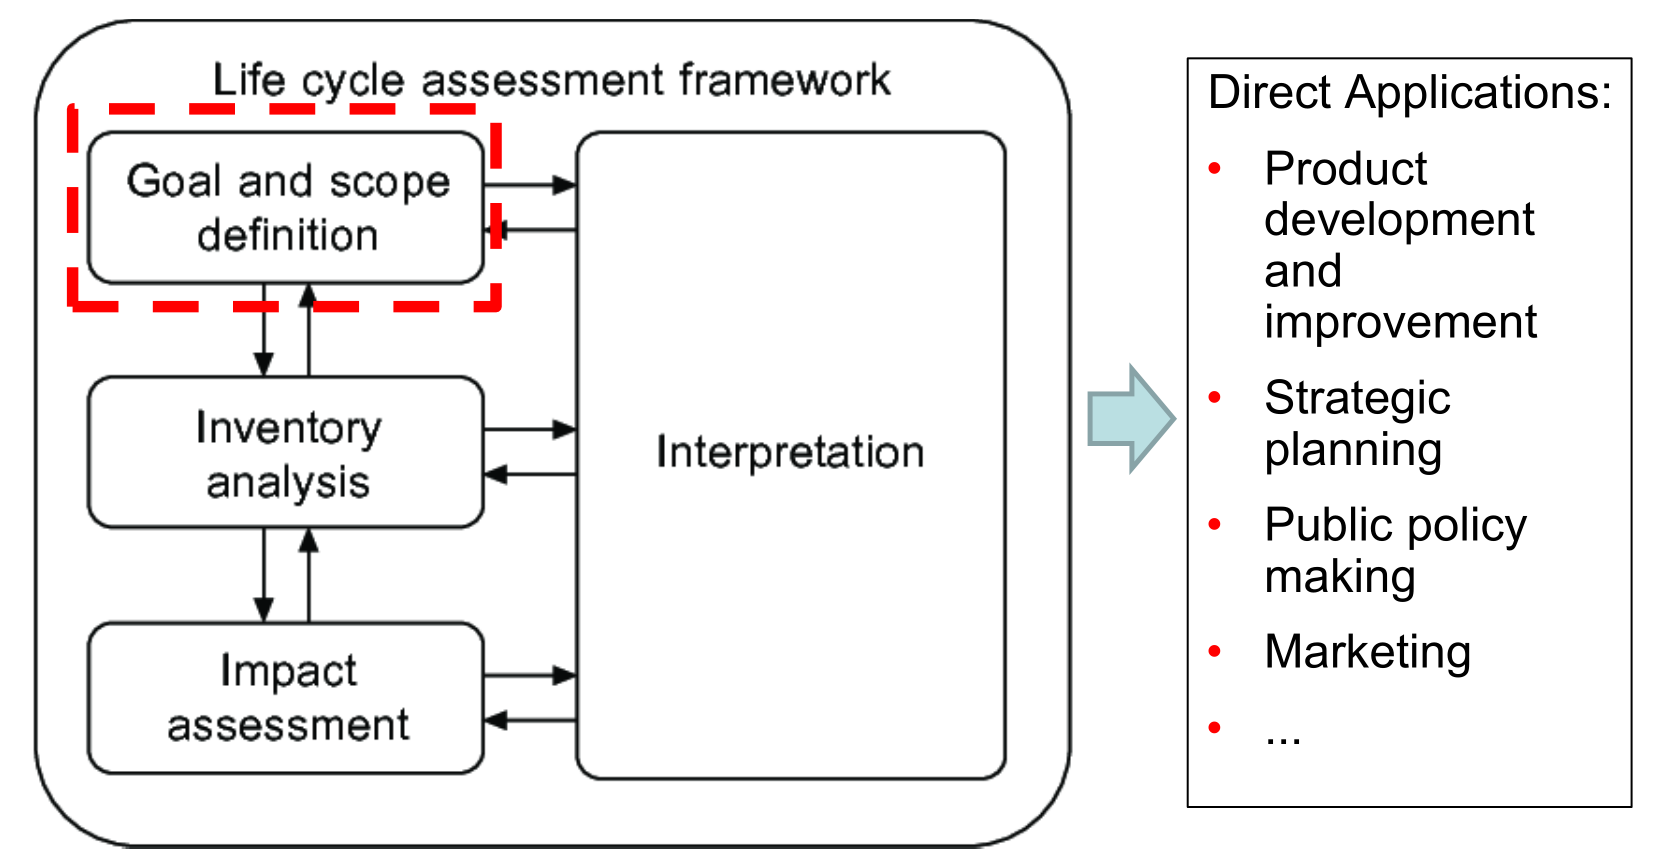
\includegraphics[width=0.8\linewidth]{img/iso_life_cycle_assessment}
\end{figure}

\subsubsection{Goal and Scope Definition}
Questions to be answered:
\begin{itemize}
	\item What is being studied?
	\item What is the aim of the study?
	\item Who is addressed?
\end{itemize}

Central terms are \textbf{functional unit} which is to what quantity or benefit the environmental impacts are related, and what performance is being compared, and \textbf{system boundaries} which is what is and what is not taken into account.

\begin{definition}
	\textbf{System boundary} is the functional unit of a product system and is a quantified description of the performance requirements that the product system fulfils. This unit should relate as much as possible to the functions of the product rather than the physical product. It has to be the same for all compared product systems.
\end{definition}

System boundaries define which parts of the life cycle and which processes belong to the analysed system. They are the interface between a product system and its environment or other product systems.

\subsubsection{Inventory Analysis}
This is a compilation of all material and energy flows of the functional unit in the defined system within the system boundaries.
\begin{figure}[H]
	\centering
	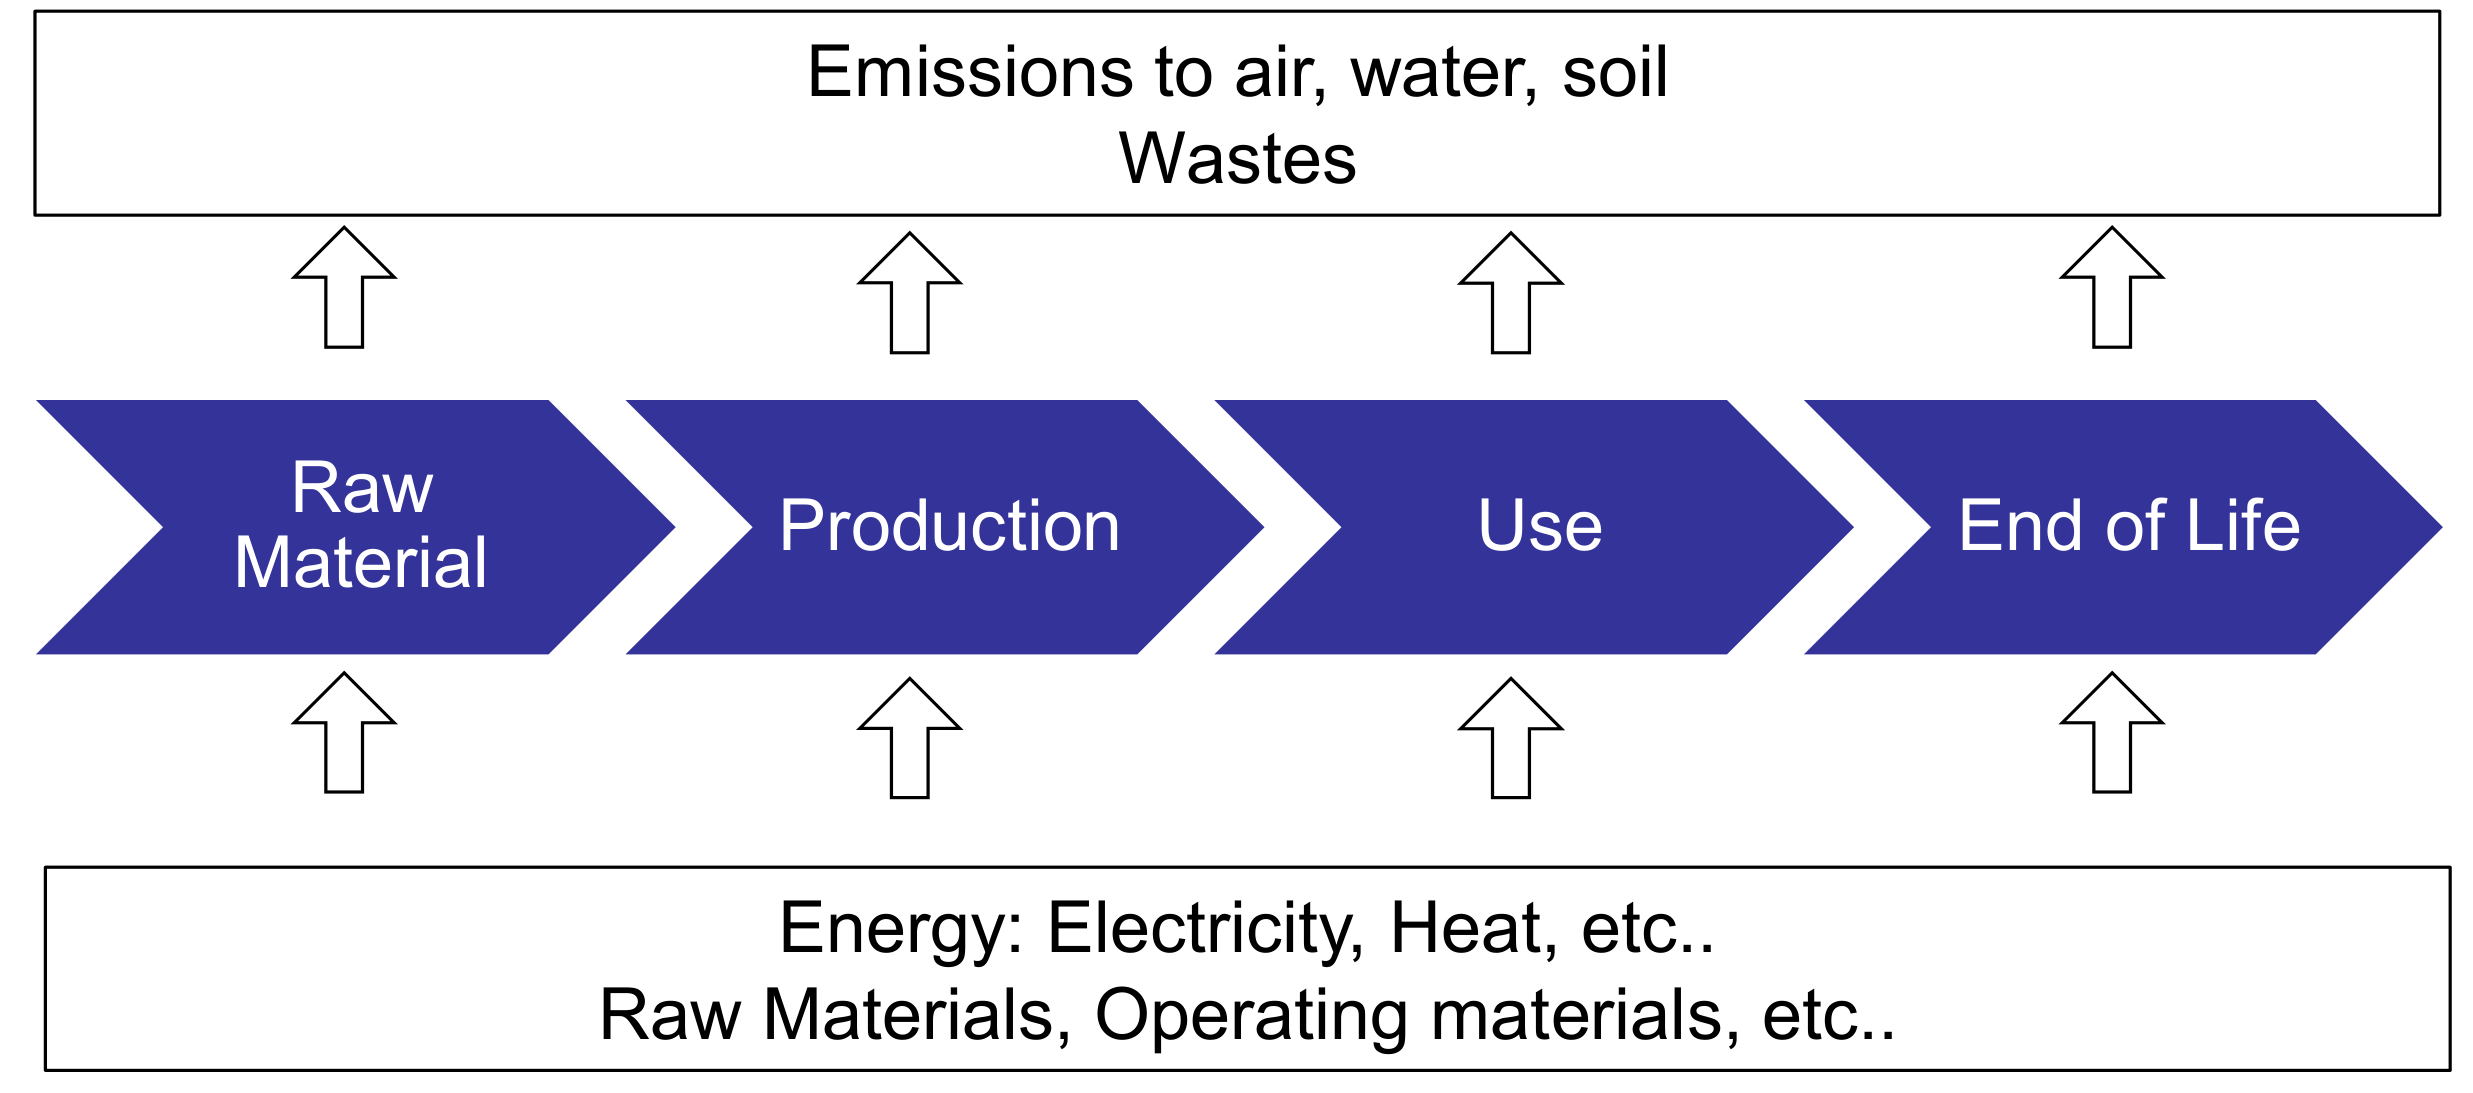
\includegraphics[width=0.8\linewidth]{img/inventory_analysis}
	\caption{Inventory analysis contributors}
	\label{fig:inventoryanalysis}
\end{figure}

\subsubsection{Impact Assessment}
The goal of the impact assessment is to trace the emissions or resource requirements along their path from the source to where the effect occurs in the environment. The difficulty is to not to lose yourself in the details and to determine a final impact.

\paragraph{$\text{CO}_2$ or Carbon Footprint} Converts climate-impacting emissions into $\text{CO}_2$ equivalents according to IPCC. It neglects other, possibly more direct, environmental impacts.

\paragraph{Ecological Scarcity Method} The method compares the current environmental load (actual quantity) with the load considered permissible from a socio-political point of view (tolerance quantity). The higher the actual to tolerance ratio, the higher the eco-factor of a substance (emission, resource consumption). It is measured in environmental damage points.

\begin{figure}[H]
	\centering
	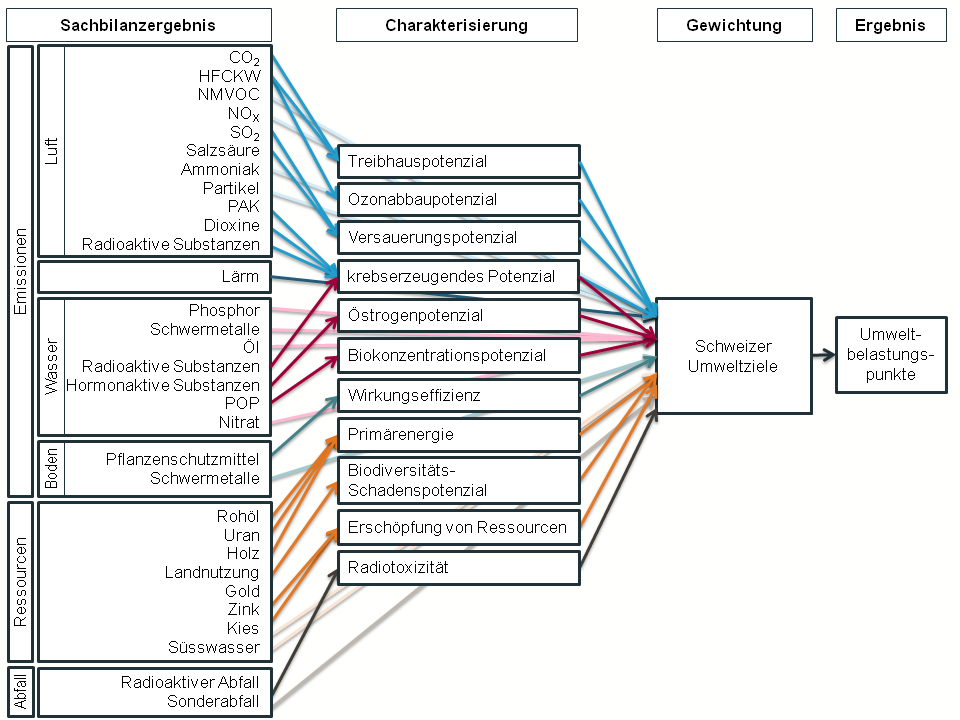
\includegraphics[width=0.8\linewidth]{img/ecological_scarcity_method_example}
	\caption{Example of impacts considered with the environmental scarcity method.}
	\label{fig:ecologicalscarcitymethodexample}
\end{figure}

\subsection{Interpretation and Evaluation}
Critical examination of all preceding steps including the identification of parameters relevant for the result, a check of consistency and completeness and a sensitivity analysis. Ask yourself if the values are correct and their certainty, which findings can be derived, what could be relevant causes for this result, and what consequences can be drawn.

\subsection{Strengths and Limits of an LCA}
\textbf{Strengths}
\begin{itemize}
	\item Comprehensive regarding substances and their impact\\
	LCA does not focus on individual problems or substances, but tries to take into account as large a number of effects as possible.
	\item Comprehensive regarding life cycle phases of products\\
	LCA considers the entire life cycle and thus also looks "behind the scenes".
	\item Quantitative\\
	LCA quantifies the environmental impact. This allows the results to be integrated into management processes and linked to economic parameters, for example.
\end{itemize}

\vspace{1em}
\noindent
\textbf{Limits}
\begin{itemize}
	\item Not all impacts are considered (for example Noise or Smell)
	\item No distinction between local and global impact
	\item Quantification can pretend accuracy, which is not given
\end{itemize}

Life cycle assessments show the environmental impacts and their relevance for a specific system. Therefore, there is no such thing as the right LCA. But there are issues for which the LCA is the most suitable method if applied and interpreted correctly. The quality criterion for a life cycle assessment is transparency and thus traceability.

\section{Circular Economy}
We need to transition to a circular economy as the rate of consumption is much greater than the regeneration of these resources.
\begin{definition}
	\textquotedblleft The circular economy is an industrial system that is restorative by design.\textquotedblright\\
	\hspace*{1em} - Ellen MacArthur Foundation, 2013
\end{definition}

\begin{definition}
	\textquotedblleft A circular economy is an economic system aimed at eliminating waste and the continual use of resources. [...] The circular economy aims to keep products, equipment and infrastructure in use for longer, thus improving the productivity of these resources. Waste materials and energy should become input for other processes.\textquotedblright\\
	\hspace*{1em} - Geissdoerfer et al, 2017
\end{definition}

\begin{figure}[H]
	\begin{subfigure}[b]{0.48\linewidth}
		\centering
		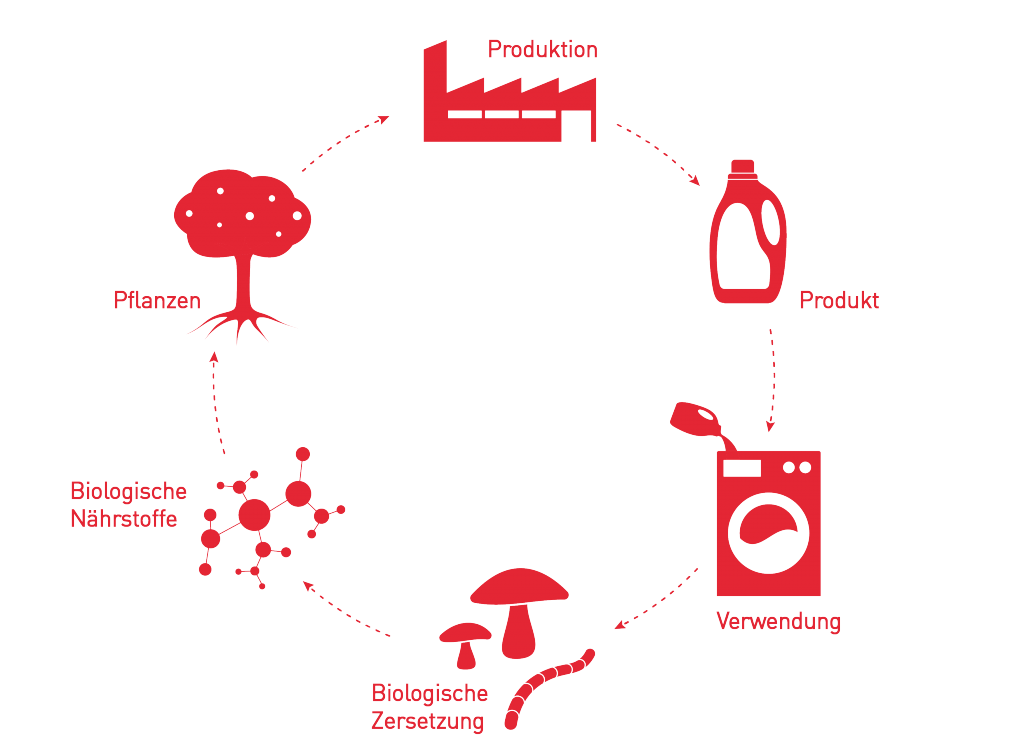
\includegraphics[width=\linewidth]{img/circular_economy_biological.png}
		\caption{Circular economy for a biological product}
	\end{subfigure}
	\hfill
	\begin{subfigure}[b]{0.48\linewidth}
		\centering
		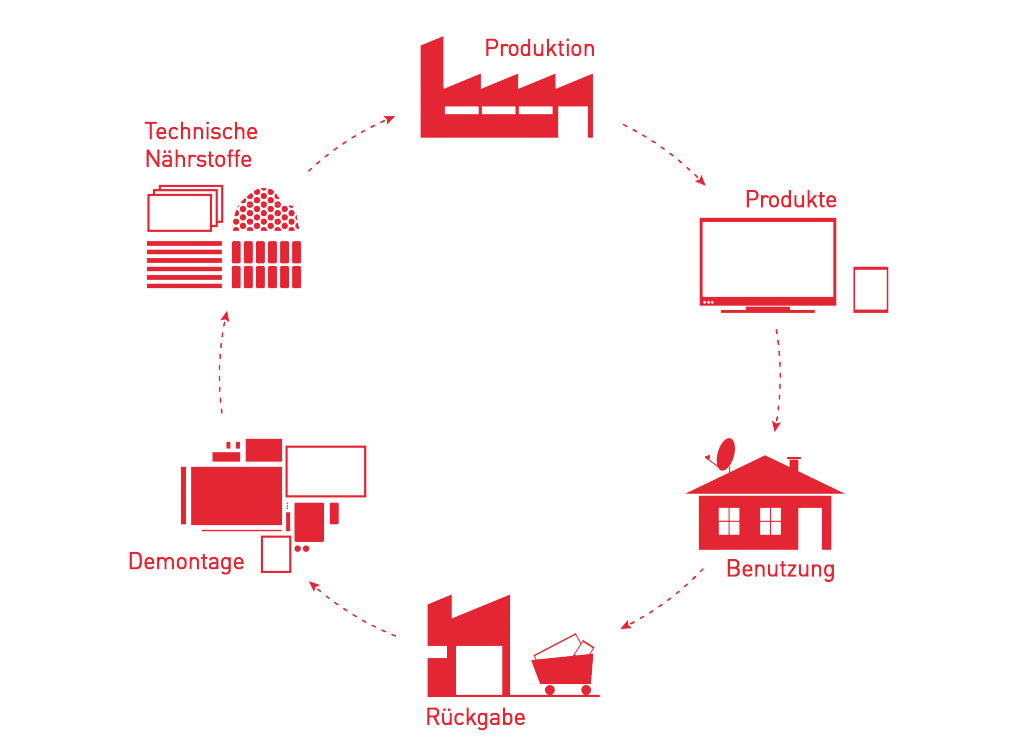
\includegraphics[width=\linewidth]{img/circular_economy_technical.png}
		\caption{Circular economy for a technical product}
	\end{subfigure}
	\caption{Source for both images: \href{https://epeaswitzerland.com/cradle-to-cradle/}{EPEA Switzerland}}
\end{figure}

\subsection{Different Sales Models}
\begin{itemize}
	\item Product as a Service\\
	Ownership replaced by 'pay as you go' and maintenance, upgrading and replacement is handled by the company.
	\item Sale with Return Option\\
	Trade-in for newer products, older equipment is refurbished and upgraded to be sold again, or sorted into rewear, reuse, recycle
	\item Rental or Subscription Model\\
	Subscription model for baby clothing and maternity wear, outgrown clothing is returned, cleaned and redistributed to another customer
	\item Sale (Starting with End-of-Life Products/Resources)\\
	Upcycling of food waste into sustainable, protein for fish, chicken, and pets
\end{itemize}

\paragraph{Coordinating Circular Value Chains through Data} Globechainis a B2B marketplace for reuse across multiple industries, like construction, hotels, offices, medical, restaurants, and retail. Organisations no longer needing assets (like furniture, equipment, or office supplies) list them on the platform, where they’re requested and collected by other companies.

\subsection{Four Types of Circular Business Model (CBM) Innovation}
\begin{itemize}
	\item CBM Transformation\\
	Modification of current business model to CBM
	\item Circular Start-up\\
	New CBM is created within company
	\item CBM Diversification\\
	Additional CBM is created in addition to continuing existing business model
	\item CBM Acquisition\\
	CBM is acquired and integrated
\end{itemize}

\subsection{Economic Potentials of Circular Business Models (CBM)}
\begin{itemize}
	\item Circular Design and Business Model gives competitive advantage
	\begin{itemize}
		\item Leverage product residual values
		\item Products are your resource stock – reduce risks of volatile markets
		\item Reduce costs by 10-30\% 
	\end{itemize}
	\item Integration and monitoring of product value chain, leads to a better understanding of product utilisation, know-how and services
	\item Services lead to more intensive and long-term customer relationships
	\item Stimulates innovation -- in product design and business models
\end{itemize}

\subsection{Risks for Negative Ecological Impacts}
Circular design often, but not always, leads to a better life cycle assessment of the product and its use. Often positive due to cycling, extending, intensifying and dematerialising.
\begin{itemize}
	\item \textbf{Extended product life-time for active products} (use phase)\\
	Older products with lower energy efficiency than state-of-the-art feature an optimal life time which is lower than the maximal life time (replacement may lead to lower overall impacts)
	\item \textbf{New materials}\\
	Trade-offs between recyclability of materials and environmental impact during production, transport, use, etc.
	\item \textbf{New technologies}\\
	New technologies can, in addition to optimizing an environmentally relevant dimension have new negative effects
	\item \textbf{Rebound effects}\\
	Reduced prices (or increase simplicity) lead to increased consumption
\end{itemize}

\subsection{Circular Economy Design Principles}
\begin{figure}[H]
	\centering
	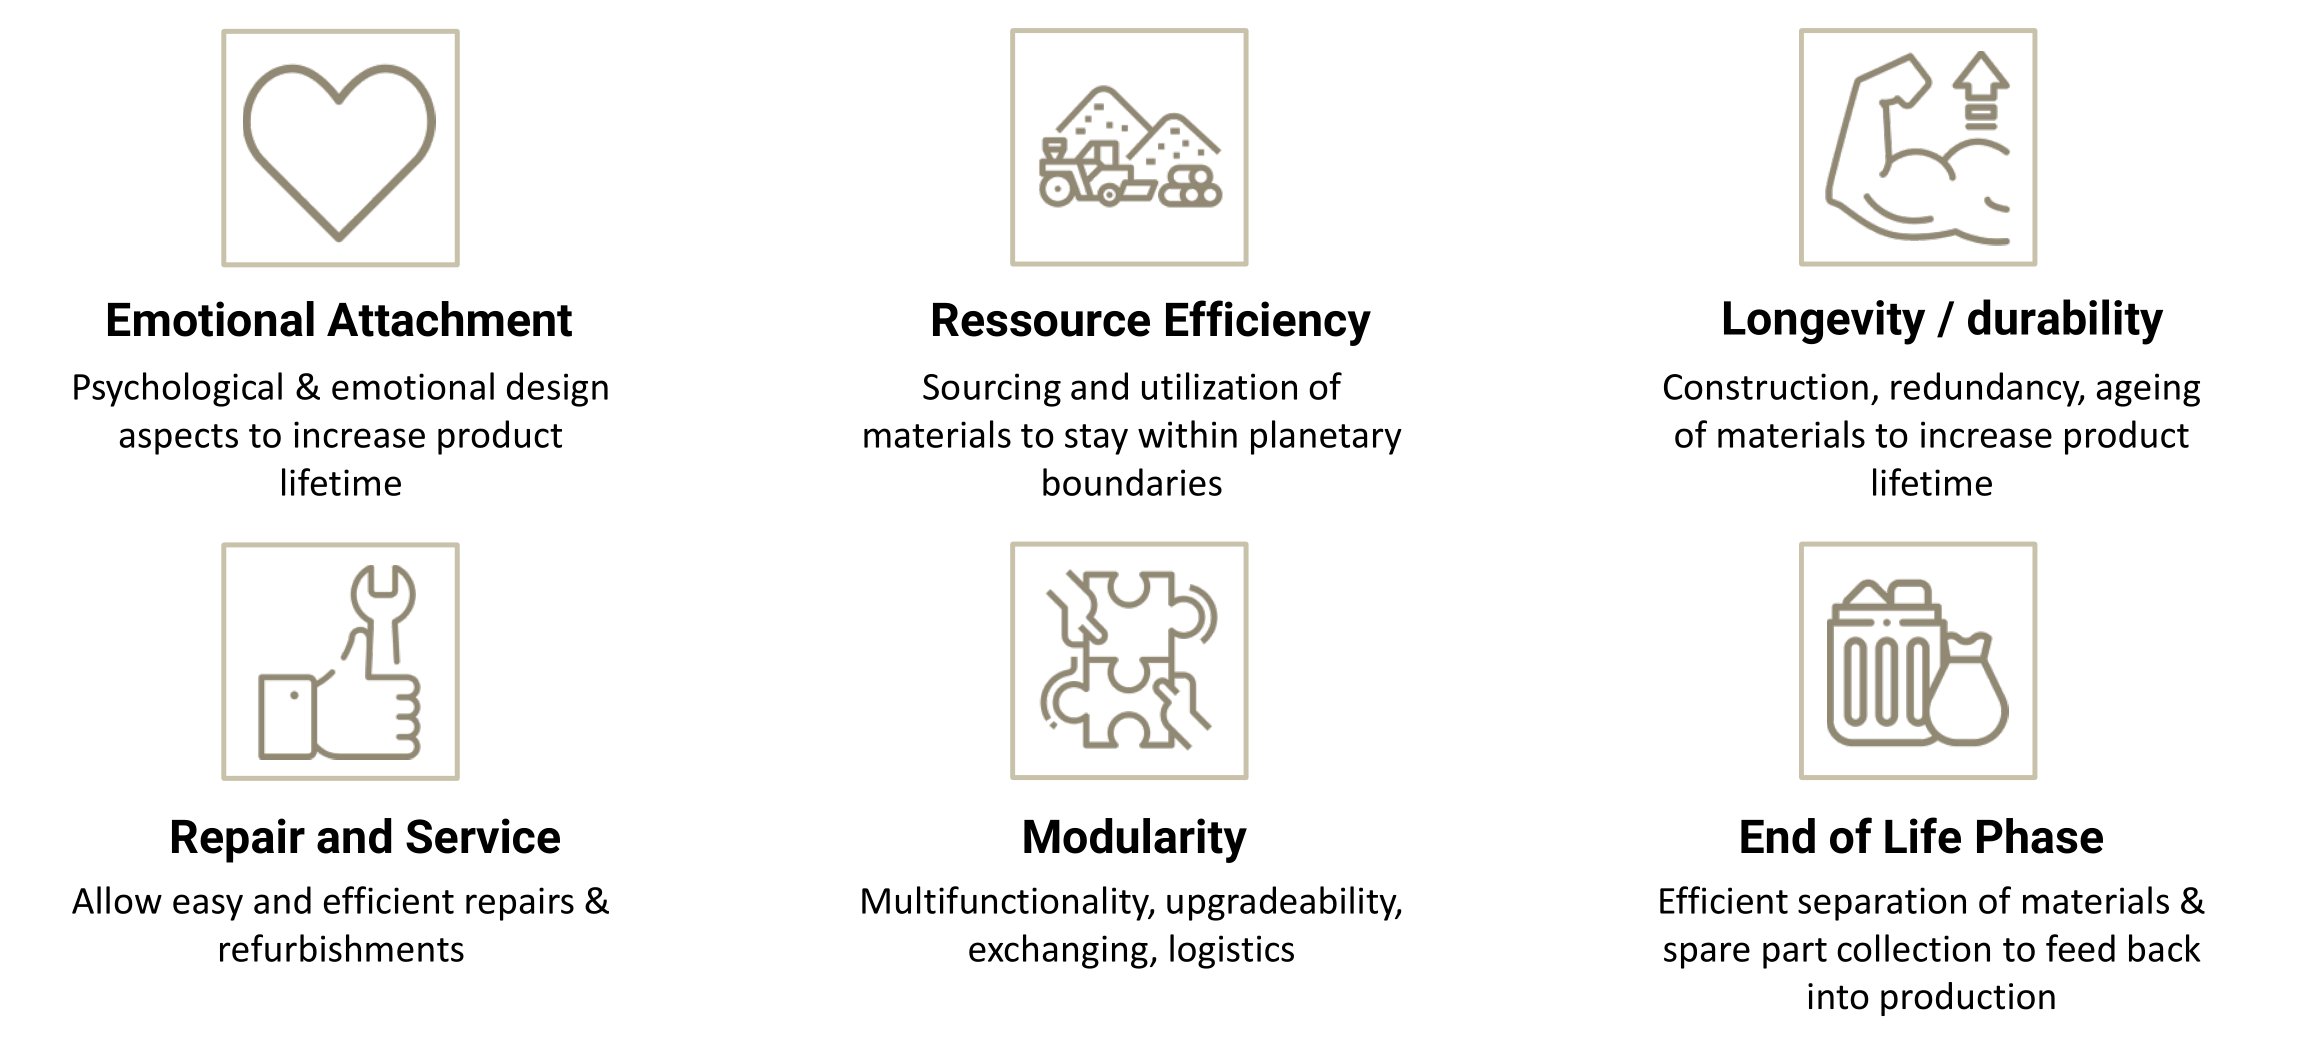
\includegraphics[width=0.8\linewidth]{img/circular_economy_design_principles}
	\caption{Source: loopi guest lecture}
	\label{fig:circulareconomydesignprinciples}
\end{figure}

\begin{itemize}
	\item \textbf{Emotional Attachment}\\
	\textbf{Interaction} You know everything about your thing -- become an expert, \textbf{Positive association} Your reminded of something you
	love, Fan culture, positive memories, \textbf{Meaningful Product} I support a cause; I am a part of something bigger, Encourage positive change, provide sense of control, feeling of changing something
	\item \textbf{Resource Efficiency}\\
	\textbf{Optimise} Reduce the size -- reduces the number of materials needed, use everything, \textbf{Secondary materials} Source from a secondary material stream and use beneficial synergies
	\item \textbf{Longevity and Durability}\\
	\textbf{Reduce moving parts} Friction between moving parts promotes wear and tear, \textbf{Ageing} Materials change with time, plan ahead, use materials that allow a graceful ageing of your product
	\item \textbf{Service and Repairability}\\
	\textbf{Easy exchange of parts} Provide easy access to fasteners and highlight them, \textbf{Let the users repair} Repairing can be fun and increases product attachment, make it easy
	\item \textbf{Modularity}\\
	\textbf{Reverse Logistics} Every part or material should return to you, establish incentives for customers to return goods, use modules for optimized transport size, \textbf{Compatibility}
	Standardisation, use the same fastening principles in every product generation, \textbf{Allow upgrades} Requirements change over time, allow easy upgrading through standardisation of the components you are using
	\item \textbf{End of Life Phase}\\
	\textbf{Avoid composite materials, Inlays and permanent joining} Separation of materials is vital for recycling, recycling has to be economically viable as it is in competition with incineration and landfills, \textbf{Collect spare parts} Some parts life longer than others
\end{itemize}

\section{Industrial Ecology (IE)}
Industrial ecology is the study of material and energy flows through industrial systems. It is concerned with the impacts that industrial activities have on the environment, with use of the planet's supply of natural resources, and with problems of waste disposal. This field approaches issues of sustainability by examining problems from multiple perspectives, usually involving aspects of sociology, the environment, economy, and technology.

\vspace*{1em}
\noindent
\textbf{Perspectives and Tools}
\begin{itemize}
	\item Life cycle thinking, complete value chains
	\item Combination of services, capital flows, material flows, and energy flows
	\item Material cycles, industrial symbioses
\end{itemize}

\section{Sustainability Strategy}
Which aspect of Sustainability is most important to focus on?
\begin{itemize}
	\item Values, Vision, Mission towards sustainable development
	\item Commitment of top management
	\item Knowledge of impacts
	\item Knowledge of stakeholder expectations
	\item Sustainability strategy
	\item Sustainability programme
	\item Reporting system to measure progress
	\item Communication (to internal and external stakeholders)
	\item Management System (integrate all above into business process)
\end{itemize}

\begin{figure}[H]
	\centering
	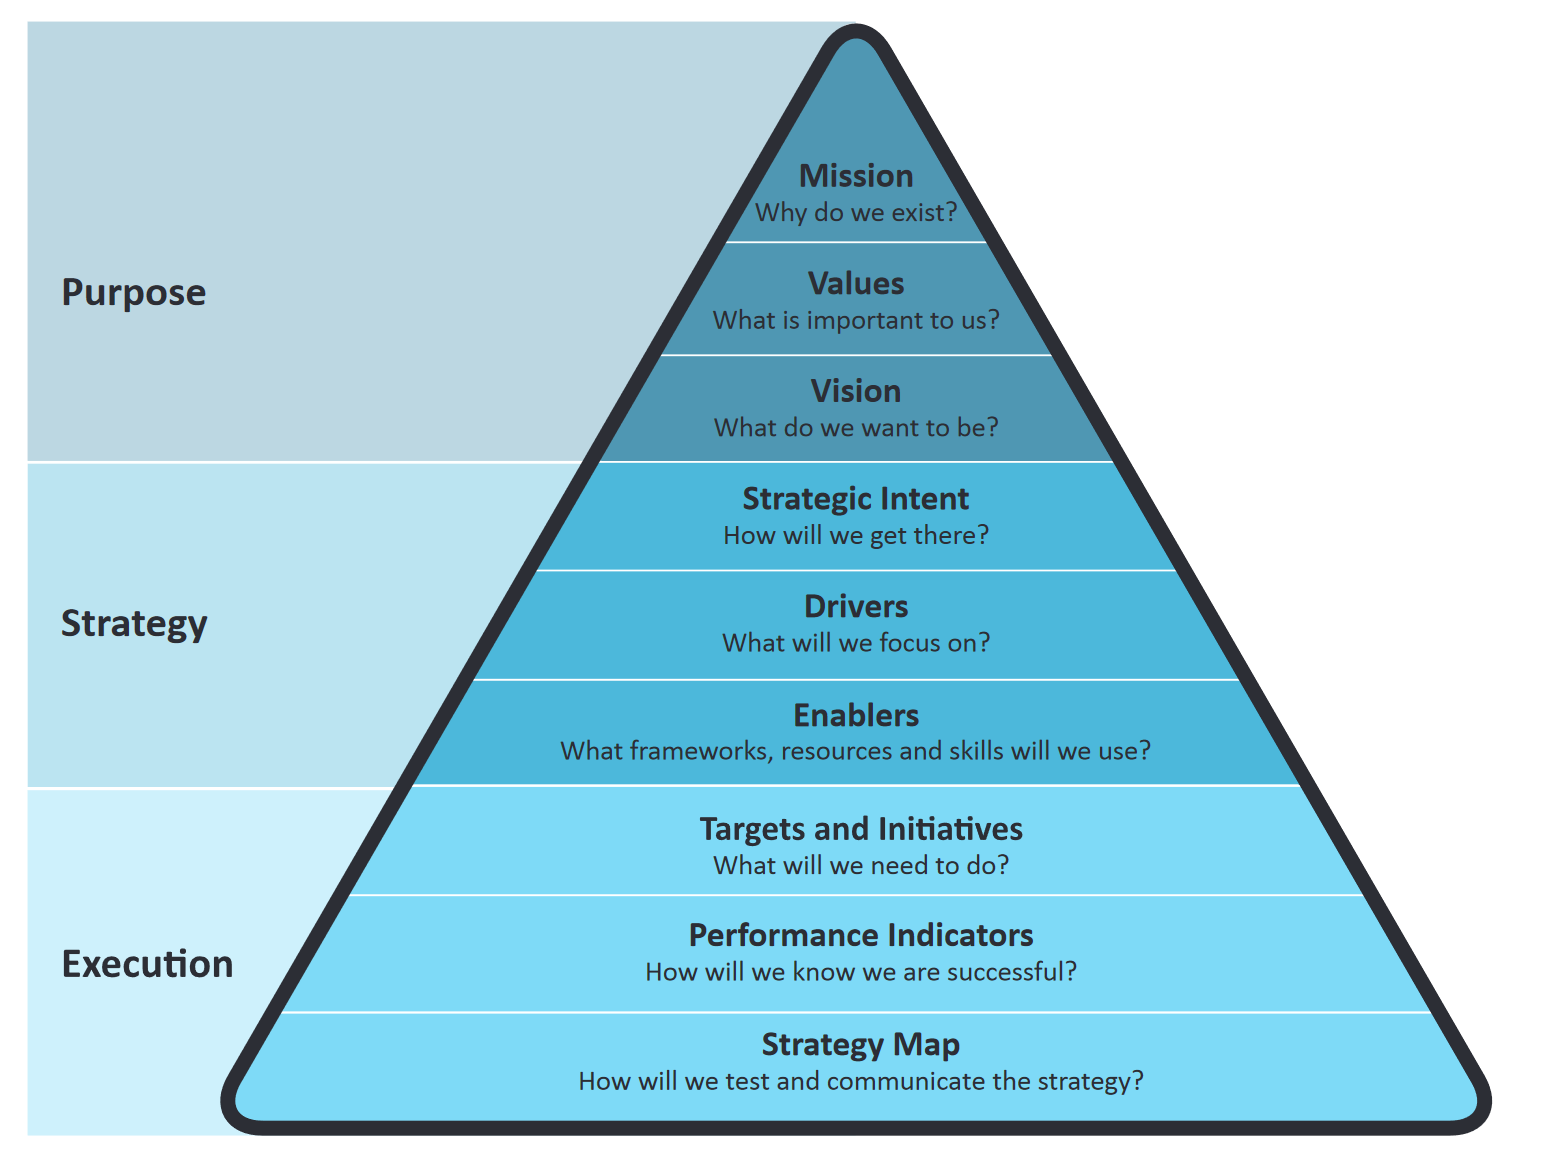
\includegraphics[width=0.6\linewidth]{img/strategy_map}
	\caption{The strategy pyramid highlighting the nine pillars of progress. "The formula for improving well-being through science consists of nine strategic pillars that together build a space where science and society meet. The pillars build sequentially on one another, creating an integrated and transparent framework in what could loosely be called a social contract." (McGuinness, Wendy, 02.2019, \textit{Report 9 – Science Embraced: Government-funded science under the microscope})}
	\label{fig:strategymap}
\end{figure}

\subsection{Stakeholder Expectations}
\begin{figure}[H]
	\centering
	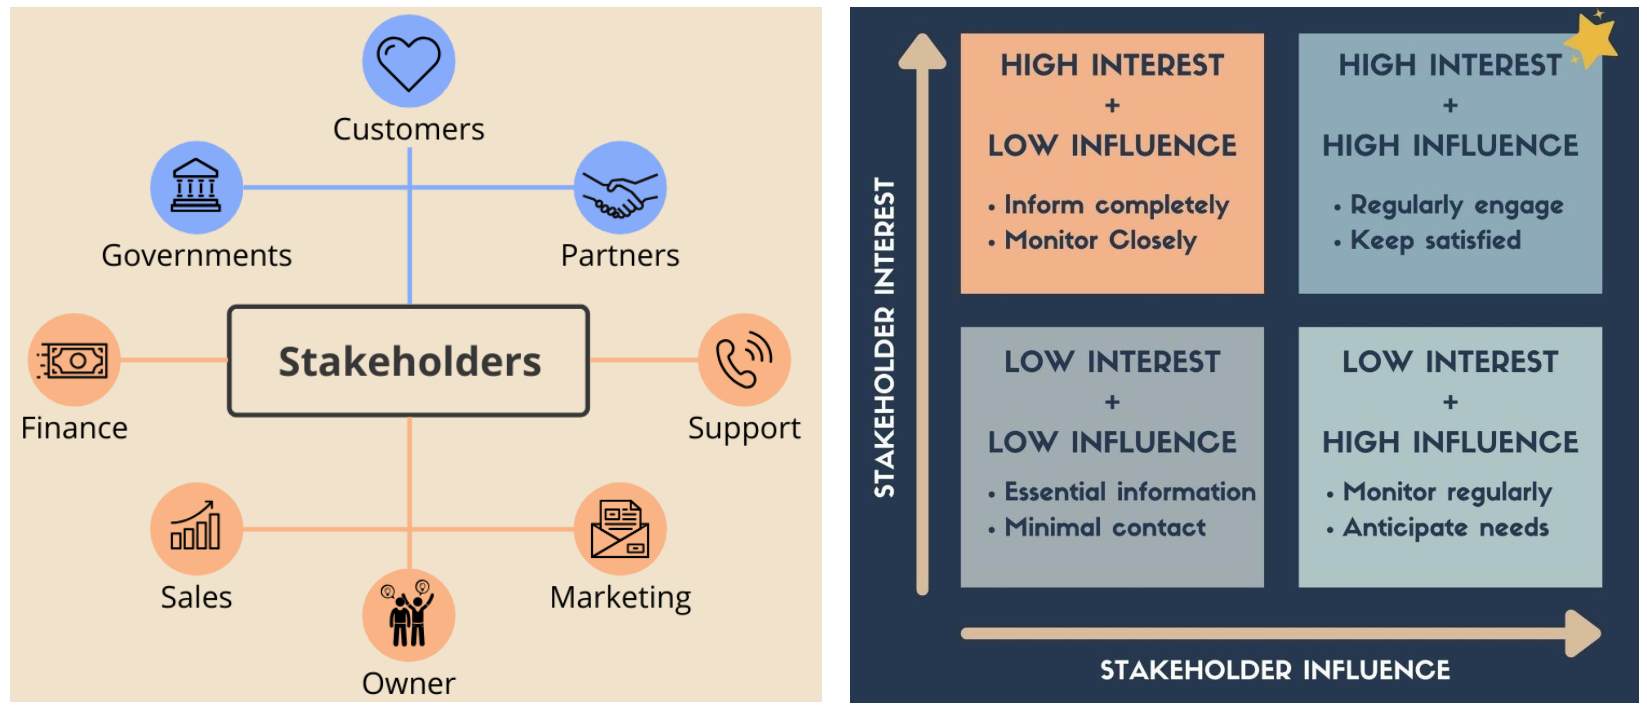
\includegraphics[width=0.7\linewidth]{img/stakeholder_expectations}
	\caption{How to identify and manage stakeholders}
	\label{fig:stakeholderexpectations}
\end{figure}
A materiality analysis is a method to identify and prioritize the issues that are
most important to an organization and its stakeholders. Process:
\begin{enumerate}
	\item Identification of topics
	\item Analysis of external expectations regarding these topics\\
	regulations, competitors, financial market, NGOs, economic environment
	\item Analysis of company impact on topics\\
	industry influence, value chain levels, geographic activity
	\item Analysis of results and validation
\end{enumerate}

\subsection{Environmental Management System}
The Environmental Management System (EMS) provides a systematic way of managing an organization's environmental affairs. This creates environmental buy-in from management and employees and assigns accountability and responsibility. An EMS assists with planning, controlling and monitoring policies in an organization. The EMS serves as a tool, or process, to improve environmental performance, and sets a framework for training to achieve objectives and desired performance. It focuses on continual improvement of the system and a way to implement policies and objectives to meet a desired result. This also helps with reviewing and auditing the EMS to find future opportunities.

\begin{figure}[H]
	\centering
	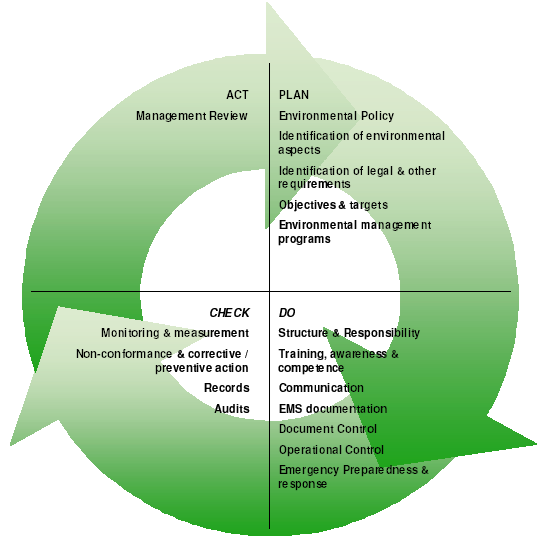
\includegraphics[width=0.6\linewidth]{img/PDCA_cycle.png}
	\caption{The integration of the \href{https://emspr.weebly.com/pdca-stages.html}{Plan-Do-Check-Act cycle} and the ISO 14001 EMS system presents a number of tasks to be carried out at each stage by environmental managers.}
	\label{fig:PDCAcycle}
\end{figure}

\end{document}
